% -----------------------------------------------------------
% Single-column working/reading version.
% Class: article 11pt A4, 2.5cm margin.
% Sage submission version: daimo-paper-en-v1.tex.
% Content identical; only the preamble and layout differ.
% -----------------------------------------------------------
\documentclass[11pt,a4paper]{article}

\usepackage[T1]{fontenc}
\usepackage[utf8]{inputenc}
\usepackage{geometry}
\usepackage{booktabs}
\usepackage{tabularx}
\usepackage{longtable}
\usepackage{array}
\usepackage{graphicx}
\usepackage{listings}
\usepackage{xcolor}
\usepackage{enumitem}
\usepackage{tikz}
\usetikzlibrary{shapes.geometric,arrows.meta,positioning,fit,backgrounds,calc}
\usepackage[colorlinks,bookmarksopen,bookmarksnumbered,citecolor=blue!50!black,urlcolor=blue!50!black,linkcolor=blue!50!black]{hyperref}

\geometry{margin=2.5cm}

\hypersetup{
  pdftitle={DAIMO: An ontology profile for governed AI model assets in dataspaces}
}

\newcommand{\code}[1]{\texttt{#1}}
\newcommand{\cq}[1]{\textsf{#1}}
\newcommand{\TODO}[1]{\textcolor{red}{\textbf{[TODO: #1]}}}
\providecommand{\keywords}[1]{\medskip\noindent\textbf{Keywords:} #1}

\newcolumntype{L}[1]{>{\raggedright\arraybackslash}p{#1}}

\lstset{
  basicstyle=\ttfamily\small,
  breaklines=true,
  columns=fullflexible,
  showstringspaces=false,
  frame=single,
  framerule=0pt,
  backgroundcolor=\color{gray!10},
  captionpos=b,
  aboveskip=0.8em,
  belowskip=0.8em
}

% Chowlk-style TikZ helpers
\tikzset{
  daimoclass/.style={rectangle, draw=black!70, fill=yellow!20, thick, rounded corners=2pt,
    minimum width=2.6cm, minimum height=0.75cm, align=center, font=\ttfamily\footnotesize,
    inner sep=3pt},
  externclass/.style={rectangle, draw=black!60, fill=blue!10, thick, rounded corners=2pt,
    minimum width=2.6cm, minimum height=0.75cm, align=center, font=\ttfamily\footnotesize,
    inner sep=3pt},
  modulebox/.style={rectangle, draw=black, fill=gray!15, thick,
    minimum width=3.2cm, minimum height=1.0cm, align=center, font=\sffamily\small\bfseries,
    inner sep=6pt},
  vocabbox/.style={rectangle, draw=black!60, fill=green!12, thick, rounded corners=3pt,
    minimum width=2.4cm, minimum height=0.7cm, align=center, font=\sffamily\footnotesize,
    inner sep=4pt},
  subclassarrow/.style={-{Triangle[open,length=3mm]}, draw=blue!70!black, thick},
  objpropertyarrow/.style={-{Latex[length=2mm]}, draw=black!80, thin},
  modulearrow/.style={-{Latex[length=2mm]}, draw=black!60, thick, dashed},
}

\title{DAIMO: An Ontology Profile for Governed AI Model Assets in Dataspaces}
\author{Edmundo de Elvira Mori Orrillo\thanks{Corresponding author: \texttt{edmundo.mori.orrillo@upm.es}.} \and Jiayun Liu \\[0.5em]
\normalsize Department of Artificial Intelligence, ETSI Inform\'aticos\\
\normalsize Universidad Polit\'ecnica de Madrid, Spain}
\date{}

\begin{document}
\maketitle

\begin{abstract}
\noindent\textbf{Abstract.}
AI models are increasingly published, negotiated, deployed, invoked, monitored, and evaluated across organisational boundaries. In dataspaces, these operations must be governed by policies, contracts, provenance records, and reproducible evaluation evidence; however, the relevant semantics are scattered across otherwise mature vocabularies. MLDCAT-AP describes machine-learning assets, DCAT supports catalog publication, ODRL represents usage policies and agreements, PROV-O captures provenance, and the Dataspace Protocol specifies contract negotiation and transfer messages. What is missing is a reusable semantic bridge that connects these vocabularies into an auditable governance chain for AI-model assets.

This article presents DAIMO (\emph{Dataspace AI Model Ontology}), an OWL~2~DL integration profile developed with the Linked Open Terms (LOT) methodology. DAIMO organises established Semantic Web vocabularies around the missing governance relations between catalogues, policies, deployments, executions, provenance records, and evaluations. Its bridge constructs include catalogued AI-asset offerings, execution authorisations, model deployments, I/O contracts, derived artefacts, audit evidence, cross-participant provenance records, shared evaluation contexts, and participant roles.

The artefact is evaluated through four complementary forms of evidence: an illustrative multi-participant dataspace scenario, OWL consistency and entailment verification, SHACL validation with structural and cross-class constraints, and twenty-three competency questions executed as SPARQL queries. The validation suite includes a negative test bench in which each cross-class invariant is exercised by a deliberately invalid graph. The resulting package contains the ontology modules, SHACL shapes, demonstrator graph, competency-question queries, validation scripts, and generated documentation.
\end{abstract}

\keywords{AI model governance; dataspace; ontology alignment; SHACL validation; LOT methodology}

% =====================================================================
\section{Introduction}\label{sec:intro}

Regulation (EU)~2024/1689, the \emph{AI Act}, requires technical documentation, execution records, lifecycle traceability, and audit evidence for high-risk AI systems~\cite{aiact}. At the same time, European dataspaces are establishing an infrastructure in which autonomous organisations publish resources, negotiate contracts, and exchange data and services through connectors such as Eclipse Dataspace Components (EDC)~\cite{edc} and protocol specifications such as the Dataspace Protocol (DSP)~\cite{dsp}. The intersection of these two developments creates a new object of semantic governance: an AI model as a federated asset whose description must support discovery, policy negotiation, authorised invocation, provenance reconstruction, and evaluation across organisational boundaries.

Semantic Web vocabularies already cover important fragments of this lifecycle. MLDCAT-AP~3.0.0~\cite{mldcatap} extends DCAT for machine-learning assets, representing models together with tasks, runs, evaluations, risks, and compute resources. DCAT~\cite{dcat2} provides the cataloguing layer; ODRL~\cite{odrl22} represents offers, permissions, prohibitions, and agreements; PROV-O~\cite{provo} records provenance over entities, activities, and agents; and DSP specifies the contract-negotiation and transfer messages implemented by dataspace connectors. Narrative documentation artefacts such as model cards~\cite{mitchell19}, factsheets~\cite{arnold19}, and datasheets~\cite{gebru21} further improve human-facing transparency.

The remaining challenge is not the absence of vocabularies, but the absence of an explicit semantic bridge between them. A machine-learning model described with MLDCAT-AP is not, by that fact alone, an offering in a federated catalog. An ODRL offer can state permissions without being tied to the model and deployment it governs. A DSP negotiation records an exchange process, but not the AI-specific evaluation context or audit evidence that may condition lawful use. A PROV bundle can group provenance descriptions without distinguishing the cross-participant governance chain of an authorised model invocation. The modelling problem is therefore relational rather than terminological: the missing semantics live at the boundaries between cataloguing, policy, deployment, execution, provenance, and evaluation. Without those boundary terms, each lifecycle fragment remains describable, but the end-to-end governance chain remains difficult to query, validate, and audit.

This article presents DAIMO (\emph{Dataspace AI Model Ontology}), an OWL~2~DL integration profile for governed AI-model assets in dataspaces. DAIMO follows a reuse-first design: it imports the semantics of established vocabularies where they already provide the required concept, and introduces a dedicated bridge construct only when the articulation between catalog, policy, execution, provenance, and evaluation cannot otherwise be represented. The resulting contribution is threefold:

\begin{itemize}[leftmargin=*]
\item a reuse-first ontology profile that preserves established vocabulary commitments while adding only the bridge constructs needed for governed AI-model exchange;
\item a requirements and validation package that links five actor needs to twenty-three competency questions, formal consistency checks, entailment analysis, structural validation, and cross-class governance invariants;
\item a reproducible multi-participant demonstrator that exercises publication, discovery, execution, auditability, evaluation, and governance-bridge queries while keeping the evidential claim bounded to executable modelling, not deployment validation.
\end{itemize}

The demonstrator uses five anonymised actor types: provider, consumer, platform operator, evaluator, and compliance actor. These actors instantiate the profile over a geospatial risk-prediction model. The demonstrator is not presented as deployment evidence; its purpose is to make the modelling commitments executable and inspectable. The rest of the article is organised as follows. Section~\ref{sec:related} reviews related work and positions the gap. Section~\ref{sec:method} describes the requirements and design decisions. Section~\ref{sec:ontology} presents the ontology. Section~\ref{sec:eval} reports the evaluation, and Section~\ref{sec:discussion} discusses limitations, integration paths, and future work.


% =====================================================================
\section{Background and related work}\label{sec:related}

DAIMO is positioned at the intersection of three bodies of work: semantic descriptions of AI models, governance vocabularies and dataspace standards, and reusable ontology-engineering practices. We review these bodies in turn, focusing on the concepts that can be reused, the gaps that remain at their boundaries, and the evaluation expectations for an ontology intended to function as an operational profile. Table~\ref{tab:reuse-matrix} then compares the relevant families of work against the five operational attributes that a profile for governed AI models must cover.

\subsection{Describing AI models}

Descriptions of AI artefacts appear at two levels of formality. \emph{Narrative} documentation---model cards~\cite{mitchell19}, factsheets~\cite{arnold19}, and datasheets for datasets~\cite{gebru21}---raised transparency standards by describing intended use, limitations, benchmark behaviour, and training conditions in natural language. These formats are valuable for human readers and qualitative accountability, but insufficient as a substrate for automated discovery, policy-based filtering, or evidence linking in machine-to-machine flows.

Structured \emph{ontologies} of the ML lifecycle cover the machine-consumable layer. EXPO~\cite{expo} offers a general ontology of scientific experiments that later work has built on. ML-Schema~\cite{mls} formalises machine-learning experiments as a reusable, lightweight schema. MEX~\cite{mex} provides an interchange vocabulary, and OntoDM~\cite{ontodm} together with DMOP~\cite{dmop} organise the data-mining domain. Souza et al.~\cite{souza19} and Schmidt et al.~\cite{schmidt21} extend the perspective towards provenance and FAIRness across the lifecycle. These ontologies offer a rigorous foundation but remain centred on the scientific experiment and the training process; none addresses the contractual dimension of exchange between autonomous participants.

The work closest to DAIMO is MLDCAT-AP~3.0.0~\cite{mldcatap} (SEMIC, 2025). MLDCAT-AP extends DCAT to describe AI models as catalogued resources with rich metadata on policy, benchmarks, evaluation, execution, risk, and compute infrastructure. DAIMO treats this representation as the AI-asset layer and concentrates on the layer that MLDCAT-AP leaves open: the act of offering a model across an organisational boundary, the governed deployment of that model as an invocable service, the authorisation of concrete executions under an agreement, and the aggregation of provenance across participants. MLDCAT-AP covers the model description; DAIMO covers the governance bridge that makes the model exchangeable, invocable, auditable, and comparable in a dataspace.

Table~\ref{tab:mldcatap-delta} makes the MLDCAT-AP relationship explicit. For each MLDCAT-AP construct most likely to co-occur with DAIMO, it records whether the construct is adopted as part of the AI-asset layer, profiled with additional conformance expectations, or complemented by a bridge construct that MLDCAT-AP does not cover. The pattern is consistent: on the AI-asset plane DAIMO preserves the SEMIC vocabulary; on the catalog-dataspace bridge it adds without overriding.

\begin{table}[t]
\small\sf\centering
\caption{Relationship between DAIMO and MLDCAT-AP~3.0.0, class by class. \emph{Adopted} means the construct remains in the MLDCAT-AP layer. \emph{Profiled} means DAIMO adds conformance expectations. \emph{Bridge extension} means DAIMO introduces a construct for the catalog-dataspace relation that MLDCAT-AP does not cover.\label{tab:mldcatap-delta}}
\begin{tabular}{@{}p{3.6cm}p{2.4cm}p{8cm}@{}}
\toprule
\textbf{MLDCAT-AP class} & \textbf{DAIMO treatment} & \textbf{Notes} \\
\midrule
\code{it6:MachineLearningModel} & Adopted + profiled & AI asset description; DAIMO requires policy, title, and identifier for governed exchange. \\
\code{it6:Task} & Adopted & Target task of a model. \\
\code{it6:Run} & Adopted + profiled & Execution record; DAIMO requires flow, algorithm, agent, timestamp, and authorisation linkage. \\
\code{it6:Flow} & Adopted & Pipeline associated with a run. \\
\code{it6:Evaluation} & Adopted & Measurement result; can be included in cross-participant provenance. \\
\code{it6:EvaluationMeasure} & Adopted & Metric type and value. \\
\code{it6:Benchmark} & Adopted & Benchmark reference used to define comparability conditions. \\
\code{it6:ComputerInfrastructure} & Adopted & Compute environment on which a deployment runs. \\
\code{it6:Hardware}, \code{it6:Library} & Adopted & Elements of the compute environment. \\
\code{it6:HarmRisk} & Adopted & Risk annotation on a model. \\
\code{it6:Modality} & Adopted & Input modality. \\
\code{it6:trainedOn}, \code{it6:testedOn} & Adopted & Training/test dataset links. \\
\midrule
\multicolumn{2}{@{}l}{\textbf{Bridge constructs absent from MLDCAT-AP and added by DAIMO}} & \\
\midrule
(no MLDCAT-AP analogue) & Bridge extension & Governed catalog offering with attached ODRL policy. \\
(no MLDCAT-AP analogue) & Bridge extension & Execution authorisation grounded in an agreement. \\
(no MLDCAT-AP analogue) & Bridge extension & Deployment relation between model, infrastructure, and invocable service. \\
(no MLDCAT-AP analogue) & Bridge extension & I/O formats and authentication conditions. \\
(no MLDCAT-AP analogue) & Bridge extension & Governable output of an authorised run. \\
(no MLDCAT-AP analogue) & Bridge extension & Compliance-oriented integrity and audit evidence. \\
(no MLDCAT-AP analogue) & Bridge extension & Provenance aggregation across participant contexts. \\
(no MLDCAT-AP analogue) & Bridge extension & Reified comparability conditions for evaluations. \\
(no MLDCAT-AP analogue) & Bridge extension & Participant role in dataspace exchange. \\
\bottomrule
\end{tabular}
\end{table}

\subsection{Governing resources and dataspaces}

Two threads of work provide the governance substrate that DAIMO composes on top of the model description. The first is the family of W3C \emph{governance vocabularies} for resources. DCAT~2~\cite{dcat2} provides the catalog primitives on which MLDCAT-AP and DAIMO rest. ODRL~2.2~\cite{odrl22} offers a consolidated model for permissions, prohibitions, obligations, offers, and binding agreements; these policy constructs are essential for describing governed model offerings and execution authorisations. PROV-O~\cite{provo} provides the provenance ontology over activities, entities, agents, bundles, and roles, and is the natural substrate for tracing individual executions and their cross-participant aggregation. Pandit and Esteves~\cite{pandit-esteves} show how ODRL combines with DPV for health-data scenarios; DAIMO transposes that pattern to the AI domain. These vocabularies are mature and widely adopted but domain-agnostic: none is specific to AI, and none is specific to dataspaces.

The second thread is the emerging set of \emph{dataspace standards} that describe the exchange itself. Franklin et al.~\cite{franklin05} framed \emph{dataspaces} as a response to persistent heterogeneity, and Otto et al.~\cite{otto19} and Cappiello et al.~\cite{cappiello22} turn data sovereignty, contracts, and controlled interoperability into explicit design assumptions. The Dataspace Protocol~\cite{dsp} is the W3C-CG specification that defines catalog, contract-negotiation, and transfer-process messages; Eclipse Dataspace Components~\cite{edc} is its reference implementation. One distinction deserves emphasis: EDC is a Java execution framework, not an ontology. The semantics that EDC implements come from DSP (protocol), ODRL (policies), and DCAT (catalog); only a handful of concepts are EDC-specific extensions, and DAIMO uses the participant-context notion only to anchor aggregated provenance to an administrative context. Work on federated ecosystems such as ConSolid~\cite{werbrouck24} further shows that the Semantic Web is evolving towards multi-actor scenarios where governance and interoperability must be designed jointly.

\subsection{Reusable and executable ontology engineering}

A third body of work informs how an ontology profile should be engineered and evaluated. Recent operational ontologies increasingly combine modular design, explicit reuse, public documentation, competency questions, and executable validation artefacts. RePlanIT~\cite{kurteva} models digital product passports for ICT equipment and validates the ontology through SHACL and expert-oriented use cases. GloSIS~\cite{palma} operationalises soil information at global scale through a modular profile aligned with SOSA/SSN and ISO~28258. FATO~\cite{fato} shows how domain literature, expert input, and competency questions can be combined when a single expert group is insufficient for sector-wide requirements. NutriLink~\cite{nutrilink} grounds its ontology in a motivating scenario and shows how competency questions become concrete query patterns. ANNO~\cite{anno} and the SAE J3016 autonomous-driving ontology~\cite{sae-onto} illustrate the value of explicit ontological commitments when domain terminology is dense and standard-driven. The Explanation Ontology~\cite{explanation-ontology} is especially relevant to DAIMO because it treats AI outputs, users, and explanatory artefacts as connected resources and evaluates the model through use cases and competency questions. Woods et al.\ connect ontology engineering with natural-language processing for industrial maintenance activities~\cite{woods}. Bareedu et al.\ derive SHACL validation rules from OPC UA industry standards~\cite{bareedu24}. Ferranti et al.\ formalise Wikidata property constraints through SHACL and SPARQL~\cite{ferranti}. Robaldo and Batsakis~\cite{robaldo} examine the interplay between SHACL validation and inference on the Time Ontology, and Penteado et al.~\cite{penteado23} study methodologies for publishing linked open government data. Taken together, these works indicate that a practically useful ontology should not only define classes and properties. It should make the full chain from requirements, reuse decisions, alignments, validation constraints, examples, documentation, and reproducibility conditions inspectable.

\begin{table*}[t]
\small\sf\centering
\caption{Reuse matrix: families of related work against the five operational attributes that a profile for governed AI models must cover. $\bullet$ = primary coverage; $\circ$ = partial coverage; --- = not covered.\label{tab:reuse-matrix}}
\begin{tabular}{@{}lccccc@{}}
\toprule
\textbf{Family / artefact} & \textbf{Publication} & \textbf{Policy} & \textbf{Invocation} & \textbf{Traceability} & \textbf{Evaluation} \\
\midrule
Model cards, factsheets, datasheets~\cite{mitchell19,arnold19,gebru21} & $\circ$ & --- & --- & --- & $\circ$ \\
ML-Schema, MEX, OntoDM, DMOP~\cite{mls,mex,ontodm,dmop} & --- & --- & --- & $\circ$ & $\bullet$ \\
MLDCAT-AP 3.0.0~\cite{mldcatap} & $\bullet$ & $\circ$ & --- & $\bullet$ & $\bullet$ \\
DCAT 2~\cite{dcat2} & $\bullet$ & --- & $\circ$ & --- & --- \\
ODRL 2.2~\cite{odrl22} & --- & $\bullet$ & --- & --- & --- \\
PROV-O~\cite{provo} & --- & --- & --- & $\bullet$ & $\circ$ \\
DSP / EDC~\cite{dsp,edc} & $\circ$ & $\circ$ & $\bullet$ & --- & --- \\
\midrule
\textbf{DAIMO} (this work) & $\bullet$ & $\bullet$ & $\bullet$ & $\bullet$ & $\bullet$ \\
\bottomrule
\end{tabular}
\end{table*}

% =====================================================================
\section{Methodology and requirements}\label{sec:method}

DAIMO was developed with the Linked Open Terms (LOT) methodology~\cite{lot22} because the contribution is not a stand-alone upper ontology but an integration profile whose adequacy depends on traceable requirements, disciplined reuse, and reproducible validation. We instantiated LOT in five activities: define the operational setting, elicit competency questions from that setting and from relevant specifications~\cite{gruninger95}, map each question to reusable vocabularies where possible, introduce bridge constructs only for unmet requirements, and validate the resulting artefact through reasoning, SHACL constraints, negative tests, and executable queries. The subsections below report these activities in the order in which they shaped the ontology.

\subsection{Illustrative scenario}\label{sec:scenario}

The illustrative scenario is used as a requirements instrument rather than as evidence of field deployment. It abstracts a recurrent dataspace situation in which five anonymised actor types exchange a geospatial risk-prediction model: \emph{Provider~A} (research organisation publishing the model), \emph{Consumer~B} (municipal consumer invoking predictions), \emph{Platform~C} (operator of the federated dataspace), \emph{Evaluator~D} (scientific evaluator publishing comparative measurements), and \emph{Compliance~E} (governance body auditing the chain). Together these actors expose the lifecycle tasks a catalogue-dataspace bridge must support: publishing a model as a governed asset, discovering it under policy and quality constraints, invoking a deployment, tracing execution evidence across participants, and comparing evaluation results under reproducible conditions. The evaluation section later instantiates the same scenario to make the requirements and validation artefacts executable.

\subsection{Requirements specification}\label{sec:method-req}

The requirements were derived from three complementary sources: the illustrative scenario, the public specification of MLDCAT-AP~3.0.0, and the public documentation of Eclipse Dataspace Components and the Dataspace Protocol. The resulting twenty-three competency questions are grouped by actor and lifecycle stage. Category R (registration and publication, five questions) concerns the provider's need to publish a model as a governed asset with identity, licence, policy, and invocation contract. Category D (discovery and selection, four questions) captures the consumer's need to locate a suitable model by task, domain, policy, and quality threshold. Category E (execution and auditability, five questions) concerns invocation, operational traces, and evidence reconstruction. Category V (evaluation and reproducibility, five questions) covers comparisons under homogeneous evaluation conditions. Category G (governance bridge, four questions) isolates cross-actor questions that cannot be answered by the reused vocabularies without additional bridge semantics. Table~\ref{tab:actors} summarises the actor-category mapping; Table~\ref{tab:req-trace} traces each requirement family to the modelling commitments that answer it; the full set of twenty-three questions in natural language appears in the competency-question appendix.

\begin{table*}[t]
\small\sf\centering
\caption{Actors involved in the illustrative scenario and the competency-question categories derived from them.\label{tab:actors}}
\begin{tabular}{@{}p{3.5cm}p{2cm}p{7cm}p{2.5cm}@{}}
\toprule
\textbf{Actor} & \textbf{Category} & \textbf{Need} & \textbf{CQs} \\
\midrule
Model provider & R & Publish a model as a governed asset with identity, licence, policy, and invocation contract & \cq{CQ-R1}--\cq{CQ-R5} \\
Model consumer & D & Discover models by task, domain, policy, and quality threshold & \cq{CQ-D1}--\cq{CQ-D4} \\
Platform operator & E & Invoke services, trace executions, and reconstruct operational evidence & \cq{CQ-E1}--\cq{CQ-E5} \\
Evaluator & V & Compare results under a shared context and inspect reproducibility & \cq{CQ-V1}--\cq{CQ-V5} \\
Governance (multi-actor) & G & Bridge offer, deployment, authorisation, and cross-participant provenance & \cq{CQ-G1}--\cq{CQ-G4} \\
\bottomrule
\end{tabular}
\end{table*}

\begin{table*}[t]
\small\sf\centering
\caption{Traceability from operational requirement to modelling commitment. The table is intended to make visible why each modelling group exists and which evaluation artefact exercises it.\label{tab:req-trace}}
\begin{tabular}{@{}p{3.2cm}p{4.3cm}p{4.2cm}p{2.8cm}@{}}
\toprule
\textbf{Requirement family} & \textbf{Question the profile must answer} & \textbf{Primary DAIMO commitment} & \textbf{Evidence} \\
\midrule
Publication & Is this model a governed asset in a particular catalog context? & Governed offering record linking model, publisher, catalog context, and applicable policy. & CQs R1--R5, G1 \\
Discovery & Can a consumer filter models by task, domain, policy, and evaluation threshold? & MLDCAT-AP model/task/evaluation semantics plus policy links and evaluation context. & CQs D1--D4 \\
Invocation & Which service, authentication method, and I/O contract apply to a selected model? & Deployment description plus service and I/O-contract commitments, allowing several endpoints per hosted model. & CQs E1, G2 \\
Authorisation & Which agreement authorised a concrete execution by a concrete participant? & Negotiated agreement linked to the participant role and execution it covers. & CQs E2, G3; INV-2, INV-4 \\
Auditability & Can a governance actor reconstruct artefacts, evidence, and provenance across contexts? & Derived artefact, evidence record, and cross-participant provenance bundle. & CQs E4, E5, G4; INV-1 \\
Evaluation & Are measurements comparable under the same task, dataset version, protocol, and seed? & Shared evaluation context capturing task, dataset version, protocol, and seed. & CQs V1--V5 \\
\bottomrule
\end{tabular}
\end{table*}

The question set also fixes the intended reasoning profile. Eleven of the twenty-three questions require explicit reasoning, either through subclass paths, subproperty chains, or SPARQL aggregation; the remaining twelve are answerable without inferencing. This split is important for an integration ontology. It shows where formal semantics add interoperability value while keeping the ordinary discovery and reporting questions executable on standard SPARQL endpoints.

The non-functional requirements constrain both modelling content and publication quality. The artefact is constrained to OWL~2~DL for decidability and HermiT compatibility, is released under CC-BY~4.0 (Apache~2.0 for validation code), and uses persistent URIs under \url{https://w3id.org/pionera/daimo} with content negotiation, WIDOCO documentation~\cite{widoco}, and accessible SHACL validation. A reuse-by-default rule binds the modelling work: each DAIMO term must justify why none of DCAT, DCAT-AP, MLDCAT-AP, ODRL, PROV-O, DSP, or the EDC extension already covers the required meaning.

\subsection{Core design decisions}\label{sec:method-design}

Three structural decisions shape the rest of the design.

\paragraph{Decision~1: reuse preferentially.} DAIMO preserves the conceptualisations of established vocabularies whenever they already capture the intended meaning. MLDCAT-AP remains responsible for the model, task, run, pipeline, evaluation, and compute-environment layer; DCAT remains responsible for cataloguing and service description; and ODRL remains responsible for policy offers and agreements. DAIMO intervenes only where these layers must be connected for governed exchange.

Introducing DAIMO-specific equivalents for any of these would violate the principle of minimal ontological commitment~\cite{gruber95} and fracture the DCAT-AP ecosystem without adding expressive power. A new class is therefore justified only when the union of the reused vocabularies leaves a concrete gap that prevents answering at least one competency question.

\paragraph{Decision~2: separate three complementary planes.} The architecture distinguishes three planes that DAIMO connects but does not replace. The dataspace exchange plane covers participant contexts, catalogue exchange, and protocol-level interaction. The governance-operation plane covers offers, agreements, authorisations, and evidence records that make exchange auditable. The AI-asset plane covers model descriptions, tasks, runs, evaluations, and compute environments. DAIMO binds these planes at their lifecycle boundaries instead of redefining the vocabularies that own them.

\paragraph{Decision~3: one class per gap, not per theme.} Given reuse preference, each class introduced by DAIMO must justify its existence by a concrete gap in the union of the reused vocabularies and by at least one competency question that cannot be answered without it. Strict application of this criterion produces nine top-level classes (\code{AIAssetOffering}, \code{ParticipantRole}, \code{ModelDeployment}, \code{IOContract}, \code{ExecutionAuthorization}, \code{DerivedArtifact}, \code{CrossParticipantProvenanceRecord}, \code{AuditEvidence}, and \code{SharedEvaluationContext}) plus five role subclasses. Any candidate class failing both conditions simultaneously is discarded.

% =====================================================================
\section{The DAIMO ontology}\label{sec:ontology}

\subsection{Modular architecture and metrics}\label{sec:scope}

The ontology specification follows directly from the requirements in Section~\ref{sec:method}. The competency questions delimit five tasks: publication as a catalogue record, policy-and-quality-sensitive discovery, invocation through typed services, traceability of individual executions, and contextualised evaluation. Responsibilities outside this boundary, such as detailed training pipelines, fine-grained privacy-policy semantics, or formal derivation theory, already belong to mature vocabularies. DAIMO therefore contributes the boundary constructs needed to make those vocabularies interoperate when an AI model circulates between autonomous participants.

The implementation is decomposed into three Turtle modules, each serving a distinct adoption need. The \textbf{core module} (\code{daimo-core.ttl}) contains the fourteen DAIMO classes, twenty-nine object properties, eight datatype properties, the global disjointness axioms, and the property characterisations (functional, asymmetric, inverse) that capture TBox-level type invariants. The \textbf{alignment module} (\code{alignment.ttl}) encapsulates the seven \code{rdfs:subClassOf} and six \code{rdfs:subPropertyOf} declarations that connect DAIMO to reused vocabularies, plus minimal declarations of external terms with \code{rdfs:seeAlso} pointers to their source specifications. The \textbf{SHACL module} (\code{daimo-shapes.ttl}) contributes eighteen \code{sh:NodeShape}s: nine structural shapes, three conformance shapes over reused classes, and six cross-class invariants expressed with \code{sh:SPARQLConstraint}. Because the SHACL module is declared as an independent \code{owl:Ontology} with its own \code{owl:versionIRI}, the validation layer can evolve without forcing a new logical vocabulary release.

\begin{figure}[t]
\centering
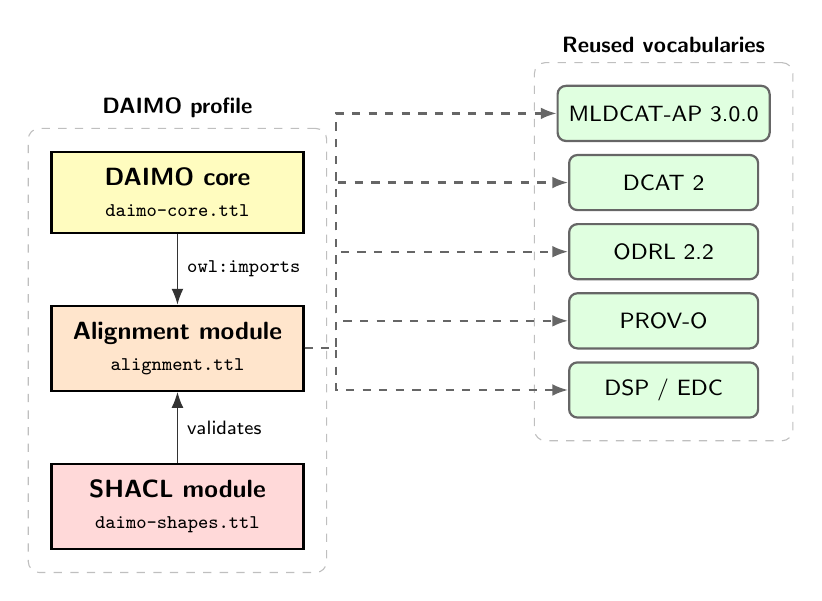
\begin{tikzpicture}[node distance=0.9cm and 0.7cm]
  % Three DAIMO modules (vertical stack on the left)
  \node[modulebox, fill=yellow!25] (core) {DAIMO core\\\scriptsize\normalfont\code{daimo-core.ttl}};
  \node[modulebox, fill=orange!20, below=of core] (align) {Alignment module\\\scriptsize\normalfont\code{alignment.ttl}};
  \node[modulebox, fill=red!15, below=of align] (shapes) {SHACL module\\\scriptsize\normalfont\code{daimo-shapes.ttl}};

  % Five reused vocabulary layers (vertical stack on the right)
  \node[vocabbox, right=3.2cm of core, yshift=1.0cm] (mldcat) {MLDCAT-AP 3.0.0};
  \node[vocabbox, below=0.15cm of mldcat] (dcat) {DCAT 2};
  \node[vocabbox, below=0.15cm of dcat] (odrl) {ODRL 2.2};
  \node[vocabbox, below=0.15cm of odrl] (prov) {PROV-O};
  \node[vocabbox, below=0.15cm of prov] (dsp) {DSP / EDC};

  % Arrows from alignment module (the bridge) to each vocabulary
  \draw[modulearrow] (align.east) -- ++(0.4,0) |- (mldcat.west);
  \draw[modulearrow] (align.east) -- ++(0.4,0) |- (dcat.west);
  \draw[modulearrow] (align.east) -- ++(0.4,0) |- (odrl.west);
  \draw[modulearrow] (align.east) -- ++(0.4,0) |- (prov.west);
  \draw[modulearrow] (align.east) -- ++(0.4,0) |- (dsp.west);

  % Core imports alignment (used by consumers who want inference)
  \draw[objpropertyarrow] (core.south) -- node[right, font=\scriptsize\sffamily] {\code{owl:imports}} (align.north);
  \draw[objpropertyarrow] (shapes.north) -- node[right, font=\scriptsize\sffamily] {validates} (align.south);

  % Legend
  \begin{scope}[on background layer]
    \node[fit=(core)(shapes), draw=gray!50, dashed, inner sep=8pt, rounded corners] (daimobox) {};
    \node[above=0.0cm of daimobox, font=\sffamily\footnotesize\bfseries] {DAIMO profile};
  \end{scope}
  \begin{scope}[on background layer]
    \node[fit=(mldcat)(dsp), draw=gray!50, dashed, inner sep=8pt, rounded corners] (vocbox) {};
    \node[above=0.0cm of vocbox, font=\sffamily\footnotesize\bfseries] {Reused vocabularies};
  \end{scope}
\end{tikzpicture}
\caption{Modular architecture of DAIMO and reused vocabularies. Yellow, orange, and red boxes denote the three DAIMO modules (core, alignment, shapes); green boxes denote the reused vocabularies. Dashed arrows from the alignment module carry the \code{rdfs:subClassOf} and \code{rdfs:subPropertyOf} declarations. The core module imports alignments for inference; the SHACL module validates data against the combined TBox.}
\label{fig:architecture}
\end{figure}

Table~\ref{tab:metrics} summarises the size and expressivity of the artefact, computed from the ontology files and validation reports (Section~\ref{sec:eval}). The numbers let a reader compare DAIMO with previously published ontologies in the same family.

\begin{table}[t]
\small\sf\centering
\caption{DAIMO artefact metrics verified against package files.\label{tab:metrics}}
\begin{tabular}{@{}p{4.6cm}r@{}}
\toprule
\textbf{Dimension} & \textbf{Value} \\
\midrule
Declared logical profile & OWL 2 DL \\
DAIMO top-level classes & 9 \\
DAIMO subclasses (\code{ParticipantRole}) & 5 \\
Total DAIMO-specific classes & 14 \\
Object properties (\code{owl:ObjectProperty}) & 29 \\
Datatype properties (\code{owl:DatatypeProperty}) & 8 \\
Functional properties (\code{owl:FunctionalProperty}) & 28 \\
Asymmetric properties (\code{owl:AsymmetricProperty}) & 5 \\
Explicit inverse pairs (\code{owl:inverseOf}) & 5 \\
\code{rdfs:subClassOf} to externals & 7 \\
\code{rdfs:subPropertyOf} to externals & 6 \\
Named disjointness axiom & 1 \\
Total \code{sh:NodeShape}s & 18 \\
\quad completeness (one per DAIMO class) & 9 \\
\quad conformance over reused classes & 3 \\
\quad cross-class SPARQL invariants & 6 \\
Competency questions & 23 \\
OOPS! pitfalls (Critical/Important/Minor) & 0 / 0 / 2 \\
\bottomrule
\end{tabular}
\end{table}

\TODO{A complementary OntoMetrics-style table (Prot\'eg\'e plugin) is missing, breaking axiom counts down by type: SubClassOf, EquivalentClasses, DisjointClasses, ObjectPropertyDomain, ObjectPropertyRange, FunctionalObjectProperty, AsymmetricObjectProperty, InverseObjectProperties, SubDataPropertyOf, DataPropertyDomain, DataPropertyRange, AnnotationAssertion, etc. RePlanIT \S5.2 and most ontology-journal papers report this table; it gives the reviewer a quantitative measure of axiomatic richness independent of class and property counts.}

\subsection{Classes and alignments}\label{sec:classes}

The class layer is organised around lifecycle boundary objects rather than around broad AI-governance themes. The nine top-level classes, together with the five \code{ParticipantRole} subclasses, are the minimal set required by the competency questions under the reuse rule introduced above. Table~\ref{tab:classes} summarises each class, its axiomatic alignment to reused vocabularies, and the competency questions it supports. Figure~\ref{fig:classes} gives the corresponding structural view.

\begin{table*}[t]
\small\sf\centering
\caption{DAIMO classes, axiomatic alignments, and the competency questions they answer.\label{tab:classes}}
\begin{tabular}{@{}p{4cm}p{3cm}p{6cm}p{2.2cm}@{}}
\toprule
\textbf{Class} & \textbf{Alignment} & \textbf{Role} & \textbf{CQs} \\
\midrule
\code{daimo:AIAssetOffering} & \code{dcat:CatalogRecord} & Catalog record that publishes a model as a governed offer in a dataspace; carries an ODRL policy via \code{daimo:hasOfferPolicy}. & R1, R2, R5, G1 \\
\code{daimo:ParticipantRole} \newline (+5 non-disjoint subclasses) & \code{prov:Role} & Role a participant plays with respect to an AI asset within a dataspace context. & R5 \\
\code{daimo:ModelDeployment} & \code{prov:Entity} & Running or hosted instance of a model, exposed as a \code{dcat:DataService} over an \code{it6:ComputerInfrastructure}. & E1, E3, G2 \\
\code{daimo:IOContract} & (no external alignment) & Minimal actionable contract: I/O formats, authentication method, optional schemas. & R4, E1, G2 \\
\code{daimo:ExecutionAuthorization} & \code{odrl:Agreement} & ODRL agreement derived from a DSP negotiation that authorises concrete executions via \code{daimo:authorizesRun}. & E2, E5, G3 \\
\code{daimo:DerivedArtifact} & \code{prov:Entity}, \code{dcat:Resource} & Governed and catalogable output produced by an execution under authorisation. & E5, G4 \\
\code{daimo:CrossParticipantProvenanceRecord} & \code{prov:Bundle} & Aggregation of activities and entities across participant contexts forming an audit narrative. & G4 \\
\code{daimo:AuditEvidence} & \code{prov:Entity} & Compliance-oriented evidence record with structured \code{spdx:Checksum}, signer, and timestamp. & E4 \\
\code{daimo:SharedEvaluationContext} & (no external alignment) & Reified comparability conditions: task, dataset, version, protocol, and random seed. & V1, V2, V3 \\
\bottomrule
\end{tabular}
\end{table*}

\begin{figure*}[t]
\centering
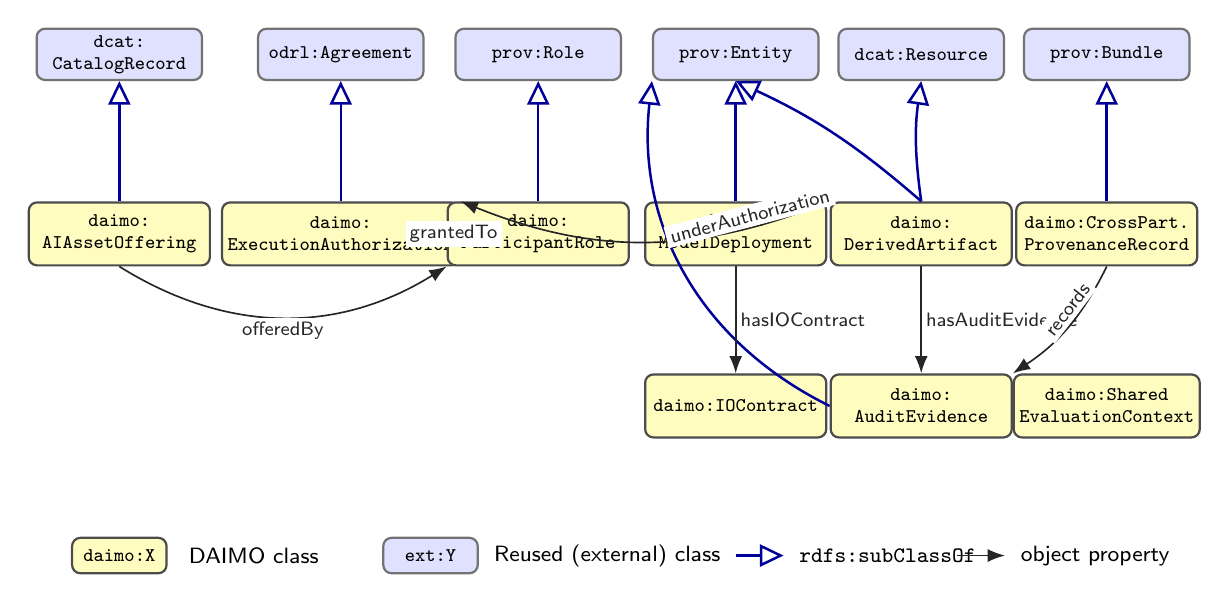
\begin{tikzpicture}[
    x=0.76cm, y=0.95cm,
    daimoclass/.style={rectangle, draw=black!70, fill=yellow!25, thick,
      rounded corners=3pt, minimum width=2.3cm, minimum height=0.8cm,
      align=center, font=\ttfamily\scriptsize, inner sep=2pt},
    externclass/.style={rectangle, draw=black!55, fill=blue!12, thick,
      rounded corners=3pt, minimum width=2.1cm, minimum height=0.65cm,
      align=center, font=\ttfamily\scriptsize, inner sep=2pt},
    subarrow/.style={-{Triangle[open,length=3mm,width=2.8mm]},
      draw=blue!60!black, line width=0.9pt},
    proparrow/.style={-{Latex[length=2.2mm]}, draw=black!85, line width=0.6pt},
    edgelab/.style={fill=white, font=\scriptsize\sffamily, inner sep=1.5pt,
      text=black!85}
  ]

  % ============ Row 1: External parents (y = 5) ============
  \node[externclass] (catrec)    at ( 0,   5) {dcat:\\CatalogRecord};
  \node[externclass] (agreement) at ( 3.7, 5) {odrl:Agreement};
  \node[externclass] (role)      at ( 7,   5) {prov:Role};
  \node[externclass] (entity)    at (10.3, 5) {prov:Entity};
  \node[externclass] (resource)  at (13.4, 5) {dcat:Resource};
  \node[externclass] (bundle)    at (16.5, 5) {prov:Bundle};

  % ============ Row 2: Main DAIMO classes (y = 2.6) ============
  \node[daimoclass] (offering) at ( 0,   2.6) {daimo:\\AIAssetOffering};
  \node[daimoclass] (auth)     at ( 3.7, 2.6) {daimo:\\ExecutionAuthorization};
  \node[daimoclass] (role_d)   at ( 7,   2.6) {daimo:\\ParticipantRole};
  \node[daimoclass] (deploy)   at (10.3, 2.6) {daimo:\\ModelDeployment};
  \node[daimoclass] (derived)  at (13.4, 2.6) {daimo:\\DerivedArtifact};
  \node[daimoclass] (bundle_d) at (16.5, 2.6) {daimo:CrossPart.\\ProvenanceRecord};

  % ============ Row 3: DAIMO classes without external parent + audit (y = 0.3) ============
  \node[daimoclass] (iocontract) at (10.3, 0.3) {daimo:IOContract};
  \node[daimoclass] (audit)      at (13.4, 0.3) {daimo:\\AuditEvidence};
  \node[daimoclass] (context)    at (16.5, 0.3) {daimo:Shared\\EvaluationContext};

  % ============ subClassOf (blue open-triangle arrows) ============
  \draw[subarrow] (offering)     -- (catrec);
  \draw[subarrow] (auth)         -- (agreement);
  \draw[subarrow] (role_d)       -- (role);
  \draw[subarrow] (deploy)       -- (entity);
  \draw[subarrow] (derived.north) to[bend right=8] (entity.south);
  \draw[subarrow] (derived.north) to[bend left=8] (resource.south);
  \draw[subarrow] (bundle_d)     -- (bundle);
  \draw[subarrow] (audit.west)   to[bend left=35]   (entity.south west);

  % ============ Object properties (black filled arrows) ============
  % offeredBy: Offering -> ParticipantRole (routed below row 2 to clear ExecAuth)
  \draw[proparrow] (offering.south) to[bend right=32]
    node[edgelab, below, pos=0.5] {offeredBy}
    (role_d.south west);

  % grantedTo: ExecAuth -> ParticipantRole (direct horizontal, no obstruction)
  \draw[proparrow] (auth.east) --
    node[edgelab, midway] {grantedTo}
    (role_d.west);

  % underAuthorization: DerivedArtifact -> ExecAuth (routed above row 2, clears all middle boxes)
  \draw[proparrow] (derived.north west) to[bend left=22]
    node[edgelab, above, pos=0.2, sloped] {underAuthorization}
    (auth.north east);

  % hasIOContract: ModelDeployment -> IOContract (straight down)
  \draw[proparrow] (deploy.south) --
    node[edgelab, right] {hasIOContract}
    (iocontract.north);

  % hasAuditEvidence: DerivedArtifact -> AuditEvidence (straight down)
  \draw[proparrow] (derived.south) --
    node[edgelab, right] {hasAuditEvidence}
    (audit.north);

  % records: CrossPart.ProvenanceRecord -> AuditEvidence (short diagonal)
  \draw[proparrow] (bundle_d.south) to[bend left=15]
    node[edgelab, above, pos=0.4, sloped] {records}
    (audit.north east);

  % ============ Legend (bottom row) ============
  \begin{scope}[shift={(0,-1.7)}]
    \node[daimoclass, minimum width=1.2cm, minimum height=0.45cm, inner sep=1pt]
      (lg1) at (0,0) {daimo:X};
    \node[anchor=west, font=\footnotesize\sffamily] at (1.0,0)
      {DAIMO class};

    \node[externclass, minimum width=1.2cm, minimum height=0.45cm, inner sep=1pt]
      (lg2) at (5.2,0) {ext:Y};
    \node[anchor=west, font=\footnotesize\sffamily] at (6.1,0)
      {Reused (external) class};

    \draw[subarrow] (10.3, 0) -- ++(0.8,0);
    \node[anchor=west, font=\footnotesize\sffamily] at (11.2,0)
      {\code{rdfs:subClassOf}};

    \draw[proparrow] (14.0, 0) -- ++(0.8,0);
    \node[anchor=west, font=\footnotesize\sffamily] at (14.9,0)
      {object property};
  \end{scope}

\end{tikzpicture}
\caption{Overview of the DAIMO classes (yellow) with their axiomatic alignments to the reused vocabularies (blue) via \code{rdfs:subClassOf} (open-triangle arrows), and the main profile properties that articulate the profile (labelled object-property arrows). \code{DerivedArtifact} has two external parents, \code{prov:Entity} and \code{dcat:Resource}; \code{AuditEvidence} is placed in the bottom row but is also a \code{prov:Entity}. Classes \code{IOContract} and \code{SharedEvaluationContext} carry no external alignment by design. Properties whose targets are classes of the reused vocabularies (\code{offersModel} to \code{it6:MachineLearningModel}, \code{authorizesRun} to \code{it6:Run}) are declared in Table~\ref{tab:classes} and are omitted here for readability.}
\label{fig:classes}
\end{figure*}

The absence of an external alignment is also a modelling decision. \code{IOContract} is not a \code{dcat:DataService}: a service is an accessible resource or endpoint, whereas the contract describes syntactic and authentication expectations over an exchange. Nor is it a \code{dct:Standard}, because the contract enumerates concrete invocation obligations rather than referring to an external specification. \code{SharedEvaluationContext} is likewise not an ML task. It reifies the combination under which two evaluations are comparable, rather than the abstract task those evaluations instantiate. Assigning either class a generic external parent would add little semantic value while increasing the chance of unintended entailments.

In the illustrative scenario of Section~\ref{sec:scenario}, the provider publishes three governed model offerings in a federated catalog. Each offering records which model is made available, which participant publishes it, which policy applies, and in which catalog context the offer is valid. The model selected by the municipal consumer is deployed as a hosted service with REST and gRPC endpoint descriptions, each carrying its own invocation contract. After the dataspace negotiation, the consumer obtains an authorisation associated with the executions it performs. Each execution produces a prediction artefact, and the chain is completed by audit evidence and a cross-participant provenance record spanning provider, consumer, and platform contexts.

\medskip\noindent\emph{Registration and participation.}
\code{AIAssetOffering} and \code{ParticipantRole} jointly solve the publication-side gap. MLDCAT-AP describes the model, and DCAT records catalog metadata, but neither expresses the governed act of making a model available to another dataspace participant. The offering is therefore treated as the catalog-facing record of a model in a specific dataspace, scoped by policy, publisher, target model, and participant context. \code{ParticipantRole}, with five non-disjoint specialisations, records the role a legal agent plays in relation to an asset and a dataspace context. The two classes jointly answer CQ-R1, CQ-R2, CQ-R5, and CQ-G1.

\medskip\noindent\emph{Execution plane.}
\code{ModelDeployment} and \code{IOContract} cover the invocation-side gap. DCAT supplies catalog-visible services, but it does not say which model a service hosts or which syntactic and authentication expectations a consumer must satisfy to call it. A deployment represents the running or hosted instance of a model on compute infrastructure. It may be exposed through one or several services, and each service may declare an invocation contract covering input/output format, authentication method, and optional schema references. This group answers CQ-E1, CQ-E3, and CQ-G2.

\medskip\noindent\emph{Authorisation and derivation.}
\code{ExecutionAuthorization} and \code{DerivedArtifact} cover the authorisation-to-output chain. ODRL supplies binding agreements, and PROV-O supplies general generation and derivation relations, but neither records the specific act of authorising a concrete machine-learning run or the governance-visible artefact that the run produces. The authorisation is modelled as the negotiated agreement that binds permissions to executions; the derived artefact is modelled as the governed output of such an execution. INV-1 enforces the consistency of this chain. The group answers CQ-E2, CQ-E5, CQ-G3, and CQ-G4.

\medskip\noindent\emph{Audit and provenance aggregation.}
\code{AuditEvidence} and \code{CrossParticipantProvenanceRecord} cover the auditability-across-boundaries gap. SPDX supplies checksums, and PROV-O supplies provenance bundles, but neither addresses compliance-oriented evidence that spans administrative contexts. Audit evidence combines an integrity value, a signer, and a timestamp; the cross-participant provenance record aggregates the relevant activities and entities across participant contexts, producing an audit narrative that a governance actor can traverse end-to-end. The group answers CQ-E4, CQ-G4.

\medskip\noindent\emph{Evaluation context.}
\code{SharedEvaluationContext} covers the comparability gap that plain MLDCAT-AP evaluations leave open. MLDCAT-AP records a measurement attached to a model; it does not reify the combination of task, dataset version, evaluation protocol, and random seed that makes two measurements comparable. Two evaluations sharing that context are comparable by construction; evaluations that differ on any coordinate are not. The class answers CQ-V1, CQ-V2, CQ-V3.

\medskip\noindent\emph{Justifying the principal alignments.}\label{sec:alignment-defense}
Two of the seven \code{rdfs:subClassOf} alignments carry more semantic commitment than the others. Plausible alternative modelling choices exist for both, so their justification is made explicit.

\paragraph{\code{AIAssetOffering} $\sqsubseteq$ \code{dcat:CatalogRecord}, not \code{dcat:Dataset}.} DCAT carefully distinguishes the offered resource (the \code{dcat:Dataset}, the thing of interest) from the record that describes that resource in a concrete catalog (the \code{dcat:CatalogRecord}, the metadata artefact). We align \code{AIAssetOffering} to \code{dcat:CatalogRecord} because an offering is conceptually the cataloguing record of the model in a specific dataspace, with a policy and a set of metadata specific to that context. The offering is not the model itself, whose AI-asset description remains in the MLDCAT-AP layer. A counter-reading that subsumed \code{AIAssetOffering} under \code{dcat:Dataset} would conflate two distinct entities: the model (which can appear in several catalogs with different conditions) and its offering in one specific catalog (which is one and has its own policy). This distinction is operationally relevant: the same model may appear in several offerings with distinct policies, and the property \code{daimo:offersModel}, aligned to \code{foaf:primaryTopic}, captures that the offering \emph{is about} the model without being identified with it.

\paragraph{\code{ExecutionAuthorization} $\sqsubseteq$ \code{odrl:Agreement}, not \code{prov:wasDerivedFrom odrl:Agreement}.} An execution authorisation is the specific result of a DSP negotiation that binds concrete ODRL permissions to concrete invocations, and ODRL models this binding instrument as \code{odrl:Agreement}: the equivalent of a contract between an assigner and an assignee, carrying effective permissions and restrictions. The alternative of relating an authorisation to an agreement via \code{prov:wasDerivedFrom} would treat the authorisation as a distinct artefact from the agreement and introduce a distinction ODRL does not require. Subsumption preserves the existing ODRL semantics for permissions, prohibitions, and obligations, while allowing existing ODRL-aware tools to recognise DAIMO authorisations as agreements. DAIMO adds only the bridge relation \code{daimo:authorizesRun}, which links the agreement to the \code{it6:Run}s it covers: a relation ODRL does not prescribe but the bridge to the provenance plane requires.

The remaining alignments are justified below, ordered from the most to the least contentious.

\paragraph{\code{ParticipantRole} $\sqsubseteq$ \code{prov:Role}.} PROV-O scopes \code{Role} to a qualified association inside a single activity, while the DAIMO role is scoped to a dataspace context and typically outlives any single execution. The subsumption is therefore defensible only in the \emph{is-a-kind-of} sense: a DAIMO role \emph{is} a role in the PROV sense whenever a specific activity qualifies it, and the scope difference is captured by the additional property \code{daimo:inContext} linking the role to an \code{edc:ParticipantContext}. A less committal alternative would be \code{skos:related} to \code{prov:Role}, which we rejected because it would prevent reasoners from classifying DAIMO roles as PROV roles when they do qualify an association. We accept the tighter subsumption with the understanding that contexts extending beyond a single activity are an additional constraint, not a contradiction.

\paragraph{\code{ModelDeployment} $\sqsubseteq$ \code{prov:Entity}.} A deployment is a persistent artefact over which activities happen (model loading, inference, logging), not an activity itself. Modelling it as \code{prov:Activity} would force each deployment to carry \code{startedAtTime}/\code{endedAtTime}, which fits a run but not a long-lived hosted instance. Aligning it to \code{prov:Entity} lets the deployment-model relation act as a genuine entity-to-entity link, and preserves the intuition that running a model on infrastructure produces a new governable entity rather than a new activity.

\paragraph{\code{DerivedArtifact} $\sqsubseteq$ \code{prov:Entity}, \code{dcat:Resource}.} The double subsumption reflects two complementary roles: a derived artefact is a \emph{provenance entity} produced by a run, and simultaneously a \emph{catalogable resource} that a governance actor may list, describe, and distribute. \code{prov:Entity} and \code{dcat:Resource} are compatible: DCAT itself treats \code{dcat:Resource} as the top of its resource hierarchy with no commitment against PROV. The OWL-RL closure over the demonstrator confirms that no unintended typing emerges from the double parent: the entailment-verification check inspects every inferred superclass of \code{DerivedArtifact} and raises zero warnings. The double alignment is what allows a single artefact to be cited both from a provenance bundle (as \code{prov:Entity}) and from a DCAT catalog record (as \code{dcat:Resource}).

\paragraph{\code{CrossParticipantProvenanceRecord} $\sqsubseteq$ \code{prov:Bundle}.} PROV-O offers two collection constructs: \code{prov:Bundle} (a named set of provenance descriptions with its own attribution) and \code{prov:Collection} (a set of entities with no attached provenance meta-semantics). The record is exactly the first: an attributable named grouping of provenance descriptions across several \code{edc:ParticipantContext}s. Aligning to \code{prov:Collection} would lose the meta-provenance layer that makes audit narratives inspectable (a bundle itself has a \code{wasAttributedTo} agent and a \code{generatedAtTime}); aligning to both would introduce redundancy. \code{prov:Bundle} is the right choice.

\paragraph{\code{AuditEvidence} $\sqsubseteq$ \code{prov:Entity}.} Evidence is a produced artefact (a hash value plus its signer and timestamp), not the act of producing it. The auditing activity is a separate \code{prov:Activity} instance associated with the compliance officer; \code{AuditEvidence} is what that activity generates. Aligning the class to \code{prov:Activity} would conflate the two and break INV-4-like invariants that compare authorisation validity against evidence generation time. The choice of \code{prov:Entity} keeps the activity-entity distinction that PROV relies on.

\subsection{Axiomatic foundations}\label{sec:axiomatic}

A taxonomy alone does not pin down meaning; it only names the types. DAIMO therefore combines the class hierarchy with an axiomatic infrastructure that fixes what each class is, what it is not, and how conforming instances must behave. Three complementary strata make up this infrastructure: OWL axioms over classes and properties, SHACL nodal constraints over instances, and SHACL-SPARQL cross-class invariants. The OWL stratum is described here; the SHACL strata appear in Section~\ref{sec:eval-invariants} as part of validation.

On the OWL stratum, disjointness between the nine DAIMO top-level kinds is declared through the named axiom \code{daimo:TopLevelKindsDisjointness}, an instance of \code{owl:AllDisjointClasses}. The five \code{ParticipantRole} subclasses are deliberately excluded: one legal agent may hold several roles at once (provider and operator, for instance), which reflects that roles are context-dependent rather than mutually exclusive.

The disjointness core is complemented by property characterisations. Twenty-eight properties are declared functional where the corresponding structural shape also imposes maximum cardinality, so cardinality is represented in both the logical and validation layers. Five lifecycle relations are asymmetric, which formally captures that a deployment is not the model it deploys, an authorisation does not coincide with the execution it authorises, and so on. Five inverse pairs support bidirectional traversal without forcing the publisher of the graph to materialise both directions.

The SHACL stratum splits into two families. Each DAIMO governance class carries a structural nodal shape that prescribes which properties are mandatory in a well-formed instance; these nine shapes are the syntactic guarantee that a publisher has supplied everything the semantic invariants need. Three conformance shapes (\code{OfferInDAIMOShape}, \code{MachineLearningModelInDAIMOShape}, and \code{RunInDAIMOShape}) establish which properties of reused classes are mandatory when a graph declares adherence to the DAIMO profile. The distinction between the two families is intentional: DAIMO does not override the underlying ontology, because that would fracture the ecosystem. Instead, it declares a commitment to a concrete subset of properties on the external classes, making the adherence criterion explicit without modifying the original definitions.

Above the shapes sit the six SHACL-SPARQL cross-class invariants (INV-1 through INV-6), examined in detail in Section~\ref{sec:eval-invariants}. They encode rules whose meaning cannot be expressed as a local constraint on a single shape because the rules span several classes simultaneously. Listing~\ref{lst:axioms} shows how the OWL axioms are encoded for the concrete case of \code{ExecutionAuthorization}: the subclass of \code{odrl:Agreement}, the asymmetry of \code{authorizesRun}, the functionality of its inverse, and membership in the named disjointness axiom.

\begin{lstlisting}[label=lst:axioms,caption={Core axioms around \code{ExecutionAuthorization}.}]
daimo:ExecutionAuthorization a owl:Class ;
    rdfs:subClassOf odrl:Agreement ;
    skos:definition "An ODRL agreement produced by a DSP contract
        negotiation that binds specific permissions to run invocations..."@en .

daimo:authorizesRun a owl:ObjectProperty , owl:AsymmetricProperty ;
    rdfs:domain daimo:ExecutionAuthorization ;
    rdfs:range  it6:Run .

daimo:authorizedBy a owl:ObjectProperty , owl:FunctionalProperty ;
    owl:inverseOf daimo:authorizesRun ;
    rdfs:domain it6:Run ;
    rdfs:range  daimo:ExecutionAuthorization .

daimo:TopLevelKindsDisjointness a owl:AllDisjointClasses ;
    owl:members ( daimo:AIAssetOffering
                  daimo:ExecutionAuthorization
                  daimo:ModelDeployment
                  daimo:DerivedArtifact
                  daimo:IOContract
                  daimo:AuditEvidence
                  daimo:CrossParticipantProvenanceRecord
                  daimo:SharedEvaluationContext
                  daimo:ParticipantRole ) .
\end{lstlisting}

\medskip\noindent\emph{Reuse surface.}\label{sec:reuse}
Table~\ref{tab:reuse} summarises the reused vocabularies and their concrete use. Three observations matter. First, the alignments to DCAT and ODRL target standard vocabularies rather than implementation-internal entities. Second, DAIMO maintains informative mappings to DSP through \code{skos:closeMatch} and \code{skos:related}, not subsumption: DSP is a messaging protocol rather than an asset ontology, and subsuming DAIMO classes under DSP constructs would introduce spurious typings. Third, of the EDC extension only \code{edc:ParticipantContext} appears explicitly, where it anchors aggregated provenance to an administrative context.

\begin{table*}[t]
\small\sf\centering
\caption{Vocabularies reused by DAIMO and the concrete use of each.\label{tab:reuse}}
\begin{tabular}{@{}p{2.6cm}p{5cm}p{7cm}@{}}
\toprule
\textbf{Vocabulary} & \textbf{Reused terms} & \textbf{Use in DAIMO} \\
\midrule
MLDCAT-AP 3.0.0 (\code{it6:}) & \code{MachineLearningModel}, \code{Task}, \code{Run}, \code{Flow}, \code{Evaluation}, \code{EvaluationMeasure}, \code{Benchmark}, \code{ComputerInfrastructure}, \code{Hardware}, \code{Library}, \code{HarmRisk}, \code{Modality}, \code{trainedOn}, \code{testedOn} & AI-asset plane; DAIMO does not redefine the model. \\
DCAT 2 (\code{dcat:}) & \code{Catalog}, \code{Dataset}, \code{Distribution}, \code{DataService}, \code{CatalogRecord}, \code{endpointURL} & Publication and discovery. \\
ODRL 2.2 (\code{odrl:}) & \code{Offer}, \code{Agreement}, \code{Permission}, \code{Prohibition}, \code{hasPolicy}, \code{target}, \code{assigner}, \code{assignee} & Policy, offer, and agreement. \\
PROV-O (\code{prov:}) & \code{Activity}, \code{Entity}, \code{Agent}, \code{Bundle}, \code{Role}, \code{wasGeneratedBy}, \code{wasAssociatedWith} & Provenance and roles. \\
FOAF (\code{foaf:})~\cite{foaf} & \code{primaryTopic} & Subproperty target for linking an offering record to the model it is about. \\
SPDX (\code{spdx:})~\cite{spdx} & \code{Checksum}, \code{algorithm}, \code{checksumValue} & Audit-evidence integrity. \\
SKOS (\code{skos:})~\cite{skos} & \code{definition}, \code{example}, \code{closeMatch}, \code{related} & Term documentation and non-subsumptive mappings. \\
DSP (\code{dspace:}) & \code{ContractOffer}, \code{ContractNegotiation}, \code{TransferProcess} & Informative \code{skos:closeMatch}/\code{skos:related} mappings; not subsumption. \\
EDC (\code{edc:}) & \code{ParticipantContext} & Only EDC-specific extension referenced. \\
\bottomrule
\end{tabular}
\end{table*}

Three subproperties that might seem natural (\code{authorizesRun} $\sqsubseteq$ \code{prov:used}; \code{grantedTo} $\sqsubseteq$ \code{prov:qualifiedAssociation}; \code{evidenceOf} $\sqsubseteq$ \code{prov:hadActivity}) are deliberately not declared, because each would produce unintended typings on authorisations, agents, or evidence under RDFS closure. The entailment-verification check of Section~\ref{sec:eval-engineering} catches errors of this kind.

% =====================================================================
\section{Evaluation}\label{sec:eval}

Evaluation is organised around four validation claims rather than around an implementation test log. Following the usual distinction between requirements coverage, formal correctness, constraint-based validation, and application-level usefulness~\cite{brank05}, we ask whether the profile can represent the target exchange, whether the OWL artefact is formally coherent, whether the SHACL constraints discriminate valid from invalid graphs, and whether the competency questions are executable over the materialised graph. This evidence pattern follows recent ontology papers that combine scenario grounding, formal artefact checks, and CQ or use-case validation, including RePlanIT~\cite{kurteva}, GloSIS~\cite{palma}, FATO~\cite{fato}, and the Explanation Ontology~\cite{explanation-ontology}. The complete reproducibility package accompanies the artefact.

\subsection{Illustrative demonstrator}\label{sec:eval-usecase}

The scenario introduced in Section~\ref{sec:scenario} is instantiated as a controlled reproducibility demonstrator. The resulting graph contains 225 triples, exercises every DAIMO class at least once, and provides the data over which the twenty-three competency questions of Section~\ref{sec:eval-cqs} are evaluated. All organisations, model names, dataset versions, and metric values are anonymised or synthetic. The demonstrator is not a deployment study; it is a compact instantiation used to test representational adequacy and to make the validation artefacts executable.

Provider~A publishes three governed model offerings in a federated catalogue: two versions of the same geospatial risk-prediction model and one read-only variant with a stricter policy. The offerings share task and domain descriptions but differ in the permissions attached to them. This part of the scenario exercises the distinction between a model as an AI asset and an offering as a contextual catalogue record with its own usage conditions.

The selected model is deployed on a described compute environment and exposed through two service interfaces: a REST endpoint with JSON input and bearer-token authentication, and a gRPC endpoint with protobuf and mutual TLS. The multi-endpoint usage exercises the modelling decision that a single deployment may expose several services and contracts, rather than forcing one endpoint per deployment.

Consumer~B obtains an execution authorisation with explicit validity dates, invokes the model, and receives a derived prediction artefact. The execution is linked to audit evidence containing an integrity record, signer, and timestamp, so that a governance actor can reconstruct how the artefact was produced and under which authorisation. A cross-participant provenance record aggregates the chain across provider, consumer, and platform contexts. Evaluator~D publishes two synthetic evaluation results under the same benchmark, protocol, and random seed, allowing the two model versions to be compared under shared conditions. Figure~\ref{fig:scenario} illustrates the instantiated scenario.

\begin{figure*}[t]
\centering
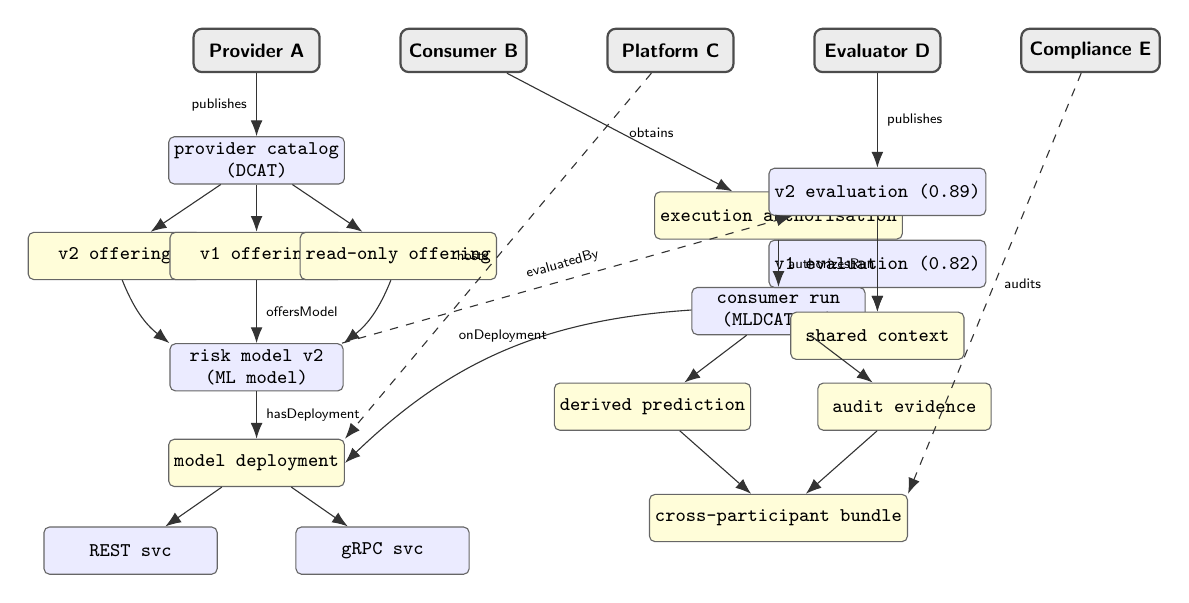
\begin{tikzpicture}[node distance=0.6cm and 0.8cm,
    instance/.style={rectangle, draw=black!60, fill=yellow!15, rounded corners=2pt,
      minimum width=2.2cm, minimum height=0.6cm, align=center, font=\ttfamily\scriptsize,
      inner sep=2pt},
    extinstance/.style={rectangle, draw=black!60, fill=blue!8, rounded corners=2pt,
      minimum width=2.2cm, minimum height=0.6cm, align=center, font=\ttfamily\scriptsize,
      inner sep=2pt},
    actorbox/.style={rectangle, draw=black!70, fill=gray!15, thick, rounded corners=3pt,
      minimum width=1.6cm, minimum height=0.55cm, align=center, font=\sffamily\scriptsize\bfseries,
      inner sep=3pt}]

  % Actors (top row, from left to right)
  \node[actorbox] (upm) {Provider~A};
  \node[actorbox, right=1.0cm of upm] (leg) {Consumer~B};
  \node[actorbox, right=1.0cm of leg] (inesdata) {Platform~C};
  \node[actorbox, right=1.0cm of inesdata] (csic) {Evaluator~D};
  \node[actorbox, right=1.0cm of csic] (gaia) {Compliance~E};

  % Publication layer
  \node[extinstance, below=0.8cm of upm] (catalog) {provider catalog\\\scriptsize (DCAT)};
  \node[instance, below=0.6cm of catalog, xshift=-1.8cm] (off1) {v2 offering};
  \node[instance, below=0.6cm of catalog] (off2) {v1 offering};
  \node[instance, below=0.6cm of catalog, xshift=1.8cm] (off3) {read-only offering};

  % Model and deployment
  \node[extinstance, below=0.8cm of off2] (model) {risk model v2\\\scriptsize (ML model)};
  \node[instance, below=0.6cm of model] (deploy) {model deployment};
  \node[extinstance, below=0.5cm of deploy, xshift=-1.6cm] (rest) {REST svc};
  \node[extinstance, below=0.5cm of deploy, xshift=1.6cm] (grpc) {gRPC svc};

  % Right side: authorization, run, derived, evidence
  \node[instance, below=1.5cm of leg, xshift=4cm] (auth) {execution authorisation};
  \node[extinstance, below=0.6cm of auth] (run) {consumer run\\\scriptsize (MLDCAT-AP)};
  \node[instance, below=0.6cm of run, xshift=-1.6cm] (derived) {derived prediction};
  \node[instance, below=0.6cm of run, xshift=1.6cm] (audit) {audit evidence};

  % Bundle (bottom)
  \node[instance, below=0.8cm of derived, xshift=1.6cm] (bundle) {cross-participant bundle};

  % Evaluation (far right)
  \node[extinstance, below=1.2cm of csic] (eval2) {v2 evaluation (0.89)};
  \node[extinstance, below=0.3cm of eval2] (eval1) {v1 evaluation (0.82)};
  \node[instance, below=0.3cm of eval1] (ctx) {shared context};

  % Arrows: publication
  \draw[objpropertyarrow] (upm) -- node[left, font=\tiny\sffamily] {publishes} (catalog);
  \draw[objpropertyarrow] (catalog) -- (off1);
  \draw[objpropertyarrow] (catalog) -- (off2);
  \draw[objpropertyarrow] (catalog) -- (off3);
  \draw[objpropertyarrow] (off2) -- node[right, font=\tiny\sffamily] {offersModel} (model);
  \draw[objpropertyarrow] (off1) to[bend right=15] (model.north west);
  \draw[objpropertyarrow] (off3) to[bend left=15] (model.north east);

  % Arrows: deployment and services
  \draw[objpropertyarrow] (model) -- node[right, font=\tiny\sffamily] {hasDeployment} (deploy);
  \draw[objpropertyarrow] (deploy) -- (rest);
  \draw[objpropertyarrow] (deploy) -- (grpc);

  % Arrows: authorization, run, derived, audit
  \draw[objpropertyarrow] (leg) -- node[right, font=\tiny\sffamily] {obtains} (auth);
  \draw[objpropertyarrow] (auth) -- node[right, font=\tiny\sffamily] {authorizesRun} (run);
  \draw[objpropertyarrow] (run) -- (derived);
  \draw[objpropertyarrow] (run) -- (audit);
  \draw[objpropertyarrow] (run) to[bend right=20] node[above, font=\tiny\sffamily] {onDeployment} (deploy.east);

  % Bundle aggregates
  \draw[objpropertyarrow] (derived) -- (bundle);
  \draw[objpropertyarrow] (audit) -- (bundle);

  % Evaluation side
  \draw[objpropertyarrow] (csic) -- node[right, font=\tiny\sffamily] {publishes} (eval2);
  \draw[objpropertyarrow] (eval2) -- (ctx);
  \draw[objpropertyarrow] (eval1) -- (ctx);
  \draw[objpropertyarrow, dashed] (model) -- node[above, font=\tiny\sffamily, sloped] {evaluatedBy} (eval2);

  % Governance audit
  \draw[objpropertyarrow, dashed] (gaia) -- node[right, font=\tiny\sffamily] {audits} (bundle.north east);
  \draw[objpropertyarrow, dashed] (inesdata) -- node[left, font=\tiny\sffamily] {hosts} (deploy.north east);

\end{tikzpicture}
\caption{Illustrative demonstrator used for validation with five anonymised participants. Grey rounded boxes on the top row are the participant contexts; yellow-shaded nodes are governance constructs introduced by DAIMO; light-blue nodes are resources described with established vocabularies. Solid arrows denote domain relations; dashed arrows show the participant role associated with an instance.}
\label{fig:scenario}
\end{figure*}

\subsection{Formal verification}\label{sec:eval-engineering}

HermiT, invoked through \code{owlready2}, confirms that the union of the core, the alignments, and the example graph is logically consistent with no unsatisfiable classes; reasoning takes 0.72~s. OWL-RL materialisation (the \code{owlrl} library) derives 1\,171 additional triples on top of 817 initial ones (1\,988 in total) in 0.27~s, with no individuals typed as \code{owl:Nothing} and no unsatisfiable subclasses.

Logical consistency is necessary but not sufficient. An ontology may be consistent and still infer, for instance, that audit evidence is a provenance activity rather than an entity produced by an activity. We therefore added an entailment-verification check over the OWL-RL closure: for each DAIMO class, the check enumerates every inferred superclass and tests it against a list of forbidden ones. The report covers the fourteen DAIMO classes (nine top-level plus five role subclasses) and raises no warning. This check complements consistency reasoning by detecting modelling-inappropriate alignments that remain logically satisfiable.

The OOPS! scanner~\cite{oops14}, queried through its REST API on the union of the core and alignments, reports zero Critical pitfalls, zero Important ones, and two Minor ones: P13 (``inverse relationships not declared'') on 34 elements with no semantically meaningful inverse, and P04 (``isolated ontology elements'') on seven locally declared external classes. Both arise from the reuse-by-default discipline the profile applies.

The final layer of formal verification targets the alignment module itself. The subclass and subproperty bridges connect DAIMO to its five parent vocabularies: DCAT, MLDCAT-AP, ODRL, PROV-O, and FOAF~\cite{foaf}. The entailment-verification check inspects the OWL-RL closure of each alignment and confirms that none produces a semantically incorrect superclass on any DAIMO governance class, raising zero warnings over the fourteen classes. Three tempting PROV-O subproperty bridges are deliberately excluded from the module for the same reason: each would have produced a forbidden typing under RDFS closure (Section~\ref{sec:axiomatic}).

\subsection{SHACL validation: structural, invariants, and negative test bench}\label{sec:eval-invariants}

The SHACL layer contains three \emph{shape} families, each answering a different validation question. Structural shapes ask whether every DAIMO-specific instance carries the mandatory properties of its class. Conformance shapes ask whether reused external classes satisfy the additional obligations that the profile imposes on them. SPARQL invariants ask whether relations across several classes remain coherent. Together, the three families move validation from local completeness to graph-level consistency: from ``is this instance well-formed?'' to ``is this graph internally coherent?''.

The nine structural shapes impose minimum completeness per DAIMO class, and the 225-triple positive graph conforms to them. The three conformance shapes add operational obligations to reused constructs: governed offers must identify their assigner and target; machine-learning models must carry policy, title, and identifier information; and execution records must include flow, algorithm, associated agent, and timestamp. Additional constraints restrict authentication methods to a closed vocabulary and evaluation protocols to recognised protocol-name patterns.

Above this structural stratum sit the six SHACL-SPARQL cross-class invariants. INV-1 guarantees consistency of the derivation-authorisation chain: every derived artefact must point to an authorisation that covers precisely the execution from which the artefact was derived. INV-2 requires the actor recorded in provenance for an execution to match the beneficiary in at least one covering authorisation. INV-3 checks data-plane coherence: a service exposed by a deployment must serve the same model the deployment declares, ruling out an endpoint that advertises one model and serves another. INV-4 ensures that an authorisation cannot justify an execution that started after the authorisation lapsed. INV-5 requires the policy attached to an offering to govern the model named in that offering. INV-6 closes the same triangle on the provider side by checking consistency between the catalogue-record attribution and the policy assigner. The positive graph conforms to all six invariants without warnings.

Listing~\ref{lst:inv5} shows the concrete encoding of INV-5 as \code{sh:SPARQLConstraint}, illustrating the \code{FILTER NOT EXISTS} pattern that captures the disjunction between policy-level and per-permission targets.

\begin{lstlisting}[label=lst:inv5,caption={INV-5 encoded as a \code{sh:SPARQLConstraint}.}]
daimo:OfferingPolicyTargetInvariant a sh:NodeShape ;
    sh:targetClass daimo:AIAssetOffering ;
    sh:sparql [
        a sh:SPARQLConstraint ;
        sh:message "INV-5 violation: offering's offersModel does not
                    appear as odrl:target of the attached policy."@en ;
        sh:prefixes daimo:_invariantPrefixes ;
        sh:select """
            SELECT $this ?model ?policy WHERE {
                $this daimo:offersModel ?model ;
                      daimo:hasOfferPolicy ?policy .
                FILTER NOT EXISTS { ?policy odrl:target ?model }
                FILTER NOT EXISTS { ?policy odrl:permission/odrl:target ?model }
            }
        """ ;
    ] .
\end{lstlisting}

Shapes that conform on the positive graph are necessary but not sufficient to show that constraints are semantically discriminating. A trivially satisfiable constraint on any graph would pass positive validation without yielding real guarantees. For this reason DAIMO also includes a companion negative graph with six deliberately invalid cases, each crafted to violate exactly one invariant. The validation workflow verifies two conditions: global validation fails, and every expected focus node appears in the report with the specific invariant's message. All six invariants fire correctly on their designated violation. This evidence complements positive validation and grounds the claim that the invariants capture operational rules.

\subsection{Competency questions}\label{sec:eval-cqs}

The twenty-three competency questions are expressed as SPARQL queries and run over the OWL-RL materialised closure of the positive graph. Table~\ref{tab:cqs} summarises coverage by category, observed row counts, and queries requiring explicit reasoning; the full set of queries appears in Appendix~\ref{app:sparql}. All twenty-three return at least one row, confirming that the demonstration graph contains the information needed to answer every question with the vocabulary, alignments, and constraints specified by the profile.

\begin{table*}[t]
\small\sf\centering
\caption{Coverage of the 23 competency questions. Each CQ returns the indicated row count over the positive graph under OWL-RL closure. Boldface marks queries that require explicit reasoning beyond plain SPARQL.\label{tab:cqs}}
\begin{tabular}{@{}p{3.3cm}p{2.6cm}p{0.8cm}p{6.3cm}@{}}
\toprule
\textbf{Category} & \textbf{Queries (rows)} & \textbf{N} & \textbf{Inference required} \\
\midrule
Registration and publication (R) & R1(3) R2(1) R3(1) R4(2) R5(2) & 5 & \textbf{R2} (\code{subPropertyOf} chain), \textbf{R5} (\code{subClassOf} path) \\
Discovery and selection (D) & D1(3) D2(2) D3(4) D4(1) & 4 & \textbf{D1} (task subtype), \textbf{D2} (policy matching) \\
Execution and auditability (E) & E1(4) E2(1) E3(2) E4(1) E5(1) & 5 & \textbf{E1} (\code{offersModel}~$\sqsubseteq$~\code{foaf:primaryTopic}), \textbf{E2} (agreement-run union) \\
Evaluation and reproducibility (V) & V1(1) V2(1) V3(2) V4(1) V5(4) & 5 & \textbf{V2}, \textbf{V3} (aggregation) \\
Governance bridge (G) & G1(1) G2(2) G3(1) G4(1) & 4 & \textbf{G3} (\code{subClassOf} reasoning), \textbf{G4} (\code{GROUP\_CONCAT} aggregation) \\
\bottomrule
\end{tabular}
\end{table*}

Two observations deserve emphasis. CQ-R2 and CQ-E1 depend on a subproperty alignment between the offering--model relation and \code{foaf:primaryTopic}; without reasoning they return no rows on a plain SPARQL engine. The dependency is documented rather than defective: the alignment makes offerings discoverable through a standard descriptive relation, a benefit that materialises only under inference. A consumer who must run those queries on a plain endpoint can materialise the closure beforehand or rewrite the queries to enumerate both properties. The second observation is that CQ-G2 returns two rows, one per endpoint of the multi-protocol REST and gRPC deployment. This confirms that modelling several services per deployment is visible in query results.

Two fragments illustrate the pattern. Listing~\ref{lst:cq-g3} shows CQ-G3 (``which authorisation authorised a specific run, and which ODRL agreement backs it?''): the query traverses the authorisation link from an execution to its agreement context, then lifts the agreement's assigner and assignee. Listing~\ref{lst:cq-v3} shows CQ-V3 (``ranking of models under the same shared evaluation context and metric''): the query joins evaluations against a fixed context, orders by metric value, and binds the model and run behind each evaluation. Both queries run over the OWL-RL-materialised closure of the demonstrator; the full query set is part of the release package.

\begin{lstlisting}[label=lst:cq-g3,caption={CQ-G3: authorisation and agreement for a specific run.}]
SELECT ?auth ?assigner ?assignee WHERE {
    ?run a it6:Run ;
         daimo:authorizedBy ?auth .
    ?auth a daimo:ExecutionAuthorization ;
          odrl:assigner ?assigner ;
          odrl:assignee ?assignee .
    FILTER (?run = <https://example.org/daimo-scenario/run-consumer-b>)
}
\end{lstlisting}

\begin{lstlisting}[label=lst:cq-v3,caption={CQ-V3: ranking of models under a shared evaluation context.}]
SELECT ?model ?metric ?value WHERE {
    ?eval a it6:Evaluation ;
          daimo:hasEvaluationContext ?ctx ;
          it6:hasMeasure ?m .
    ?m it6:metricType ?metric ;
       it6:metricValue ?value .
    ?run it6:hasEvaluation ?eval ;
         daimo:onDeployment/daimo:deploysModel ?model .
    FILTER (?ctx = <https://example.org/daimo-scenario/eval-context>)
} ORDER BY DESC(?value)
\end{lstlisting}


% =====================================================================
\section{Discussion}\label{sec:discussion}

The central contribution of DAIMO is the articulation of five lifecycle relations that are usually documented separately: publication, policy, execution, provenance, and evaluation. This articulation is what makes governed AI-model exchange queryable across organisational boundaries. Relative to recent domain ontologies such as RePlanIT~\cite{kurteva}, GloSIS~\cite{palma}, and Woods et al.~\cite{woods}, DAIMO shares an engineering ethos of reuse, executable implementation, and CQ-based evaluation, but applies it to the catalogue-dataspace boundary. Relative to earlier machine-learning lifecycle ontologies, DAIMO shares the application domain but adds the governance layer needed for dataspace exchange. Three design features support this contribution. First, entailment verification over the OWL-RL closure complements consistency reasoning by detecting modelling-inappropriate alignments that a DL reasoner may accept without contradiction. Second, cross-class SHACL-SPARQL invariants are paired with a negative test bench, so every invariant is evaluated against a case built to violate it as well as against the conforming graph. Third, reuse is formalised rather than asserted informally: external commitments are represented as explicit alignments, while three tempting PROV-O alignments are deliberately excluded because they would introduce unintended typings.

Three lines of argument bound the limitations. The first concerns \emph{semantic depth}. The I/O contract captures format and authentication method but not fine-grained semantic compatibility between model and consumer schemas, which is delegated to pipeline descriptions as Kipoi~\cite{kipoi} and TFX~\cite{tfx} do for preprocessing and pipelines. The shared evaluation context reifies task-dataset-version-protocol-seed for single-metric comparisons; heterogeneous benchmarking protocols and composite metric sets remain open. The role model folds role type into role assignment, which OntoClean recommends splitting~\cite{ontoclean}. MLDCAT-AP makes a comparable compromise in its registered-user relation, which places fine-grained contextualisation in the future-refinement horizon, not at the level of a present design error.

The second line concerns the \emph{integration commitments} and their effects on consumers who combine DAIMO with adjacent vocabularies. One provenance aggregation relation classifies recorded items as PROV activities; under RDFS reasoning, MLDCAT-AP evaluations grouped inside a cross-participant provenance record are therefore inferred as PROV activities even though MLDCAT-AP does not declare that subsumption. This does not affect the audit queries reported here, but a consumer combining DAIMO, MLDCAT-AP, and PROV-O may see surprising typings on evaluation records. Relatedly, DAIMO is not anchored to an upper ontology (BFO, GFO, DOLCE, UFO). The absence is intentional, because an integration profile is not a reference ontology. A coherent future step would be to accommodate the taxonomy to one of these upper ontologies without giving up principled reuse of the domain vocabularies that motivate DAIMO.

The third line concerns \emph{reproducibility conditions and external validation}. Reported numerical results depend on a specific reasoning profile: \code{inference=rdfs} mode in pyshacl, necessary for implied subproperties to materialise before the conformance shapes are evaluated, and the OWL-RL closure materialised before the competency queries. This dependency is documented but is a condition a consumer must know to reproduce exact results. Unlike RePlanIT and FATO, which report forms of expert or user evaluation, the present manuscript does not yet include external practitioner validation. A qualitative study with three practitioner profiles (an EDC or INESData engineer, an MLDCAT-AP/SEMIC maintainer, and an MLOps practitioner) is planned as the next phase of work. \TODO{Run the expert study: recruitment, semi-structured interview protocol, qualitative analysis, and publication of results.}

The adoption path is concrete even though a deployed pilot is not part of the present evidence. On the AI-asset side, DAIMO is designed to co-evolve with the SEMIC MLDCAT-AP dossier by preserving its model-description layer and adding only the dataspace-governance bridge. On the dataspace side, the natural integration host is Eclipse Dataspace Components: participant contexts can anchor aggregated provenance, and ODRL agreements already appear at the end of a DSP negotiation. On the governance side, DAIMO structures audit evidence around integrity records that a Gaia-X Trust Framework inspection, or an AI Act Annex IV traceability audit, would request: checksum, signer, timestamp, and linkage to a cross-participant bundle. These observations define three concrete validation paths: instantiation over a public MLDCAT-AP catalogue extract, co-deployment with an EDC connector on a federated pilot, and mapping of a high-risk AI Act use case against the six SHACL-SPARQL invariants. None of these has been executed yet; they define the short-term adoption roadmap rather than the present claims.

The relation between DAIMO and MLDCAT-AP deserves explicit delimitation. MLDCAT-AP supplies the AI-model description; DAIMO concentrates on the catalog-dataspace bridge. The four competency questions of the governance category cannot be answered with MLDCAT-AP alone, because they require an offering, a deployment, an execution authorisation, and a cross-participant provenance record. The two profiles are complementary.

Looking beyond the present artefact, DAIMO illustrates a pattern that is likely to recur wherever autonomous participants need to exchange high-value, policy-bound resources. The pattern has three recurring elements: an offering record reified above the resource itself, an authorisation reified above the permission, and a provenance bundle that crosses administrative contexts. Genomic datasets, clinical decision-support tools, digital twins, and industrial models all present analogous publication-invocation-auditing chains. DAIMO is AI-specific in what it reuses (MLDCAT-AP) but more general in the bridge constructs it adds, which can inform sibling profiles in adjacent domains.

\medskip
\noindent\textbf{Availability and FAIR compliance.}\label{sec:avail}
DAIMO is prepared as a release package under CC-BY~4.0 (ontology and documentation) and Apache~2.0 (validation scripts). The package is designed to satisfy the FAIR principles~\cite{fair}: \emph{findability} through the persistent \code{w3id.org/pionera/daimo} namespace with per-version IRIs and Dublin Core metadata; \emph{accessibility} through content negotiation across Turtle, RDF/XML, JSON-LD, and N-Triples; \emph{interoperability} through reuse of W3C and community-standard vocabularies and the OWL~2~DL profile; and \emph{reusability} through SKOS definitions and examples per term~\cite{skos}, SemVer versioning (with a deprecation policy based on \code{owl:deprecated} and \code{skos:closeMatch}), WIDOCO documentation~\cite{widoco}, and SHACL shapes that act as a data contract. Appendix~\ref{app:avail} lists the deliverable items and their locations, and the full release procedure is documented in \code{DEPLOYMENT.md} so that future maintainers can reproduce the release process.

% =====================================================================
\section{Conclusions}\label{sec:conclusion}

DAIMO contributes a governance bridge between the AI catalogue and the dataspace: offering, authorisation, deployment, derived artefact, and cross-participant provenance. The four governance-category competency questions make the gap concrete; they cannot be answered with any of the reused vocabularies alone. Entailment verification, a negative SHACL-SPARQL test bench, and the reproducible demonstrator provide complementary evidence for the profile. Future work follows from the bounded limitations: external expert validation, instantiation over a public MLDCAT-AP catalogue, refinement of I/O contracts toward schema compatibility, role-type/role-assignment separation following OntoClean~\cite{ontoclean}, and extension of shared evaluation contexts to heterogeneous benchmarking protocols. The release package is prepared under CC-BY~4.0 (ontology) and Apache~2.0 (scripts).

% =====================================================================
\begin{thebibliography}{48}

\bibitem{aiact} European Union (2024) \emph{Regulation (EU) 2024/1689 laying down harmonised rules on artificial intelligence (AI Act)}. Official Journal of the European Union.

\bibitem{edc} Eclipse Foundation. \emph{Eclipse Dataspace Components (EDC)}, control-plane documentation.

\bibitem{dsp} International Data Spaces Association (2024) \emph{Dataspace Protocol (DSP)}. W3C Community Draft.

\bibitem{mldcatap} SEMIC (2025) \emph{MLDCAT-AP 3.0.0: Machine Learning Data Catalogue Application Profile}. European Commission.

\bibitem{dcat2} Albertoni, A. et al. (2020) \emph{Data Catalog Vocabulary (DCAT) --- Version 2}. W3C Recommendation.

\bibitem{odrl22} Iannella, R., Guth, S. and Steyskal, R. (eds.) (2018) \emph{ODRL Information Model 2.2}. W3C Recommendation.

\bibitem{provo} Lebo, P., Sahoo, S. and McGuinness, D. (eds.) (2013) \emph{PROV-O: The PROV Ontology}. W3C Recommendation.

\bibitem{mitchell19} Mitchell, M. et al. (2019) Model Cards for Model Reporting. \emph{Proceedings of the Conference on Fairness, Accountability, and Transparency}.

\bibitem{arnold19} Arnold, M. et al. (2019) FactSheets: Increasing Trust in AI Services through Supplier's Declarations of Conformity. \emph{IBM Research Report}.

\bibitem{gebru21} Gebru, T. et al. (2021) Datasheets for datasets. \emph{Communications of the ACM}, 64(12):86--92.

\bibitem{expo} Soldatova, L.N. and King, R.D. (2006) An ontology of scientific experiments. \emph{Journal of the Royal Society Interface}, 3(11).

\bibitem{mls} Correa Publio, G. et al. (2018) ML-Schema: Exposing the semantics of machine learning with schemas and ontologies.

\bibitem{mex} Keet, C.M., Fernández, J.D. and Panov, P. (2016) MEX vocabulary: A lightweight interchange format for machine learning experiments. \emph{ISWC}.

\bibitem{ontodm} Panov, P., Dzeroski, S. and Soldatova, L.N. (2008) OntoDM: An ontology of data mining. \emph{ICDMW}.

\bibitem{dmop} Keet, C.M. et al. (2015) The data mining optimization ontology. \emph{Web Semantics}, 32.

\bibitem{souza19} Souza, R. et al. (2019) Provenance data in the machine learning lifecycle in computational science and engineering. \emph{WORKS}.

\bibitem{schmidt21} Schmidt, M. et al. (2021) FAIRness along the machine learning lifecycle using Dataverse in combination with MLflow. \emph{ICDE Workshops}.

\bibitem{pandit-esteves} Pandit, H.J. and Esteves, B. (in press) Enhancing Data Use Ontology (DUO) for Health-Data Sharing by Extending it with ODRL and DPV. \emph{Semantic Web}.

\bibitem{franklin05} Franklin, M., Halevy, A. and Maier, D. (2005) From Databases to Dataspaces: A New Abstraction for Information Management. \emph{SIGMOD Record}, 34(4):27--33.

\bibitem{otto19} Otto, B. et al. (2019) Reference architecture model for international data spaces. \emph{International Journal of Information Management}, 45:182--199.

\bibitem{cappiello22} Cappiello, C., Gal, A., Jarke, M., Rehof, J. and Yang, Y. (2022) Data spaces: Design, deployment, and future directions. \emph{ACM Computing Surveys}, 55(2):Article~46.

\bibitem{werbrouck24} Werbrouck, J. et al. (2024) ConSolid: A federated ecosystem for heterogeneous multi-stakeholder projects. \emph{Semantic Web}, 15:429--460.

\bibitem{kurteva} Kurteva, A. et al. (in press) RePlanIT Ontology for Digital Product Passports of ICT: Laptops and Data Servers. \emph{Semantic Web}.

\bibitem{palma} Palma, R. et al. (in press) GloSIS: The Global Soil Information System Web Ontology. \emph{Semantic Web}.

\bibitem{fato} Baryannis, G., Jia, L. and Papadakis, E. (2025) FATO: The Food Allergen Traceability Ontology. \emph{Semantic Web}.

\bibitem{nutrilink} Wu, J., Garcia, K., Mayer, S. and Albert, J. (2024) NutriLink: An Ontology for Linking Digital Receipts to Food Nutrition Information and Dietary Recommendations. \emph{Semantic Web}.

\bibitem{anno} Heuschkel, M., H\"offner, K., Schmiedel, F., Labudde, D. and Uciteli, A. (2023) The ANthropological Notation Ontology (ANNO): A core ontology for annotating human bones and deriving phenotypes. \emph{Semantic Web}.

\bibitem{sae-onto} Trypuz, R., Kulicki, P. and Sopek, M. (in press) Ontology of autonomous driving based on the SAE J3016 standard. \emph{Semantic Web}.

\bibitem{explanation-ontology} Chari, S. et al. (in press) Explanation Ontology: A General-Purpose, Semantic Representation for Supporting User-Centered Explanations. \emph{Semantic Web}.

\bibitem{woods} Woods, C. et al. (in press) An ontology for maintenance activities and its application to data quality. \emph{Semantic Web}.

\bibitem{bareedu24} Bareedu, Y.S. et al. (2024) Deriving semantic validation rules from industrial standards: An OPC UA study. \emph{Semantic Web}, 15:517--554.

\bibitem{ferranti} Ferranti, N. et al. (in press) Formalizing and Validating Wikidata's Property Constraints using SHACL and SPARQL. \emph{Semantic Web}.

\bibitem{robaldo} Robaldo, L. and Batsakis, S. (in press) On the interplay between validation and inference in SHACL. \emph{Semantic Web}.

\bibitem{penteado23} Penteado, B.E., Maldonado, J.C. and Isotani, S. (2023) Methodologies for publishing linked open government data on the Web. \emph{Semantic Web}, 14:585--610.

\bibitem{lot22} Poveda-Villalón, M., Fernández-Izquierdo, A., Fernández-López, M. and García-Castro, R. (2022) LOT: An industrial oriented ontology engineering framework. \emph{Engineering Applications of Artificial Intelligence}, 111:104755.

\bibitem{gruninger95} Gr\"uninger, M. and Fox, M.S. (1995) Methodology for the design and evaluation of ontologies. \emph{IJCAI Workshop on Basic Ontological Issues in Knowledge Sharing}.

\bibitem{widoco} Garijo, D. (2017) WIDOCO: A Wizard for Documenting Ontologies. \emph{ISWC Posters and Demonstrations}.

\bibitem{gruber95} Gruber, T.R. (1995) Toward principles for the design of ontologies used for knowledge sharing. \emph{International Journal of Human-Computer Studies}, 43(5--6):907--928.

\bibitem{foaf} Brickley, D. and Miller, L. (2014) \emph{FOAF Vocabulary Specification 0.99}. Namespace document.

\bibitem{spdx} SPDX Working Group (2022) \emph{SPDX Specification}. Version 2.3.

\bibitem{skos} Miles, A. and Bechhofer, S. (eds.) (2009) \emph{SKOS Simple Knowledge Organization System Reference}. W3C Recommendation.

\bibitem{fair} Wilkinson, M.D. et al. (2016) The FAIR Guiding Principles for scientific data management and stewardship. \emph{Scientific Data}, 3:160018.

\bibitem{brank05} Brank, J., Grobelnik, M. and Mladeni\'c, D. (2005) A survey of ontology evaluation techniques. \emph{Conference on Data Mining and Data Warehouses}.

\bibitem{shacl} Knublauch, H. and Kontokostas, D. (eds.) (2017) \emph{Shapes Constraint Language (SHACL)}. W3C Recommendation.

\bibitem{oops14} Poveda-Villalón, M., Gómez-Pérez, A. and Suárez-Figueroa, M.C. (2014) OOPS! (OntOlogy Pitfall Scanner!). \emph{International Journal on Semantic Web and Information Systems}, 10(2):7--34.

\bibitem{kipoi} Avsec, Z. et al. (2019) The Kipoi repository accelerates community exchange and reuse of predictive models for genomics. \emph{Nature Biotechnology}, 37.

\bibitem{tfx} Baylor, D. et al. (2017) TFX: A TensorFlow-based production-scale machine learning platform. \emph{KDD}.

\bibitem{ontoclean} Guarino, N. and Welty, C.A. (2002) Evaluating ontological decisions with OntoClean. \emph{Communications of the ACM}, 45(2):61--65.

\end{thebibliography}

% =====================================================================
\appendix

\section{Artefact availability}\label{app:avail}

\begin{table}[h]
\small\sf\centering
\caption{Deliverable items of the DAIMO release package and their locations.\label{tab:avail}}
\begin{tabular}{@{}p{4cm}p{11cm}@{}}
\toprule
\textbf{Item} & \textbf{Location} \\
\midrule
Persistent namespace & \url{https://w3id.org/pionera/daimo}; content negotiation configuration prepared under \code{w3id-redirect/.htaccess}. \TODO{Merge the PR on \texttt{perma-id/w3id.org} so that the namespace resolves via content negotiation.} \\
Versioned modules & Three independent ontologies (core, shapes, alignments) under \url{https://w3id.org/pionera/daimo/} with explicit \code{owl:versionIRI} and \code{owl:priorVersion} \\
Public repository & \TODO{Create public GitHub repository \texttt{pionera/daimo} by running \texttt{DEPLOYMENT.md} and include the final URL here.} \\
Versioned archival (DOI) & \TODO{Archive the first release in Zenodo and include the resulting DOI here.} \\
Serialisations & Turtle, RDF/XML, JSON-LD, N-Triples (pre-generated by WIDOCO) \\
HTML documentation & WIDOCO 1.4.25 with WebVOWL; content negotiation via \code{.htaccess} under \code{w3id-redirect/} \\
Human-readable reference & \code{ONTOLOGY-REFERENCE.md} (class by class, with \code{skos:definition}, \code{skos:example}, identity criteria, OntoClean tags) and \code{VALIDATION-MATRIX.md} \\
Release metadata & \code{CITATION.cff}, \code{.zenodo.json}, \code{CHANGELOG.md} \\
Validation package & Structural checks, OWL-RL reasoning checks, OOPS! scan, and negative test bench \\
Maintenance governance & \code{CONTRIBUTING.md} (LOT Phase 4: issue triage, pull requests, SemVer, deprecation policy) \\
\bottomrule
\end{tabular}
\end{table}

The reproducibility workflow does not require prior deployment of the persistent URL. Any user with Python~3.12 and the declared dependencies (\code{rdflib}, \code{pyshacl}, \code{owlrl}, \code{owlready2}) can run the four scripts locally and reproduce every report in \code{reports/}. The persistent URL and the DOI are additional FAIR requirements that complement but do not condition reproducibility.

\section{Competency questions}\label{app:cqs}

\subsection*{R --- Registration and publication (5)}
\begin{enumerate}[label=\arabic*., leftmargin=*]
\item \cq{CQ-R1}: Which AI models has a given provider published as governed catalog assets?
\item \cq{CQ-R2}: For a given model, which catalog offering registered it, by which publisher, and when? (requires \code{subPropertyOf} chain)
\item \cq{CQ-R3}: Licence and usage policy of a model.
\item \cq{CQ-R4}: I/O contract for the invocation interface of a published model.
\item \cq{CQ-R5}: For each offering, what concrete \code{ParticipantRole} subclass does the providing agent hold? (requires \code{subClassOf+})
\end{enumerate}

\subsection*{D --- Discovery and selection (4)}
\begin{enumerate}[label=\arabic*., leftmargin=*]
\item \cq{CQ-D1}: Which models solve a given task in a given application domain?
\item \cq{CQ-D2}: Which of those models are usable under a non-commercial policy pattern?
\item \cq{CQ-D3}: Which models expose a service endpoint, and what authentication method does each require?
\item \cq{CQ-D4}: Models reaching a minimum metric threshold under a shared evaluation context.
\end{enumerate}

\subsection*{E --- Execution and auditability (5)}
\begin{enumerate}[label=\arabic*., leftmargin=*]
\item \cq{CQ-E1}: For a given catalog offering, what service endpoint, authentication, and I/O contract apply to invoking the underlying model? (requires entailment)
\item \cq{CQ-E2}: For a given model deployment, which runs have been executed, by which agents, and under which execution authorisation?
\item \cq{CQ-E3}: Implementation, algorithm, flow, and compute infrastructure used in a run.
\item \cq{CQ-E4}: Audit evidence (hash, signer, timestamp) supporting a given run.
\item \cq{CQ-E5}: Derived artefacts produced by a run, and under which authorisation.
\end{enumerate}

\subsection*{V --- Evaluation and reproducibility (5)}
\begin{enumerate}[label=\arabic*., leftmargin=*]
\item \cq{CQ-V1}: Shared evaluation context of a given evaluation.
\item \cq{CQ-V2}: Under a shared evaluation context, highest-scoring model for a metric.
\item \cq{CQ-V3}: Ranking of models under the same evaluation context and metric.
\item \cq{CQ-V4}: For a given model, which benchmark suites has it been evaluated on?
\item \cq{CQ-V5}: Reproducibility artefacts backing an evaluation.
\end{enumerate}

\subsection*{G --- Governance bridge (4, DAIMO-specific)}
\begin{enumerate}[label=\arabic*., leftmargin=*]
\item \cq{CQ-G1}: Offerings that include a given model.
\item \cq{CQ-G2}: Deployments serving a model, with infrastructure and I/O contract.
\item \cq{CQ-G3}: Authorisation (and agreement) that authorised a specific run.
\item \cq{CQ-G4}: Full provenance bundle for a derived artefact across participant contexts.
\end{enumerate}

\section{SHACL shapes}\label{app:shapes}

The DAIMO SHACL layer contains nine structural nodal shapes, three conformance shapes over reused classes, and six cross-class SHACL-SPARQL invariants. The module \code{shapes/daimo-shapes.ttl} is itself declared as an independent \code{owl:Ontology} with its own \code{owl:versionIRI} under \url{https://w3id.org/pionera/daimo/shapes/}.

\begin{itemize}[leftmargin=*]
\item \textbf{Completeness shapes (9)}: \code{AIAssetOfferingShape}, \code{ParticipantRoleShape}, \code{ModelDeploymentShape}, \code{IOContractShape}, \code{ExecutionAuthorizationShape}, \code{DerivedArtifactShape}, \code{SharedEvaluationContextShape}, \code{AuditEvidenceShape}, \code{CrossParticipantProvenanceRecordShape}.
\item \textbf{Conformance shapes over reused classes (3)}: \code{OfferInDAIMOShape} requires \code{odrl:assigner} and \code{odrl:target} on every \code{odrl:Offer}; \code{MachineLearningModelInDAIMOShape} requires policy, title, and identifier on \code{it6:MachineLearningModel}; \code{RunInDAIMOShape} requires flow, algorithm, associated agent, and timestamp on \code{it6:Run}.
\item \textbf{Cross-class invariants (6)}: \code{DerivationAuthorizationInvariant} (INV-1), \code{RunAgentAuthorizationInvariant} (INV-2), \code{DeploymentServiceInvariant} (INV-3), \code{AuthorizationTemporalInvariant} (INV-4), \code{OfferingPolicyTargetInvariant} (INV-5), and \code{OfferingAssignerInvariant} (INV-6); all encoded as \code{sh:SPARQLConstraint}.
\end{itemize}

\section{SPARQL queries}\label{app:sparql}

The twenty-three SPARQL queries for the competency questions of Appendix~\ref{app:cqs} are released with the validation package. The validator runs each query over the OWL-RL closure of the ontology-plus-example graph and verifies that each returns at least one row. Exact counts appear in Table~\ref{tab:cqs}. CQ-G2 returns two rows (one per endpoint of the REST/gRPC multi-protocol deployment), confirming that the multi-service deployment pattern is represented in the query results.

\section{Glossary of abbreviations}\label{app:glossary}

\begin{table}[h]
\small\sf\centering
\caption{Abbreviations used in this article.\label{tab:glossary}}
\begin{tabular}{@{}p{2.2cm}p{10cm}@{}}
\toprule
\textbf{Abbrev.} & \textbf{Expansion} \\
\midrule
AI Act & Regulation (EU) 2024/1689 on artificial intelligence \\
BFO & Basic Formal Ontology \\
CQ & Competency Question \\
DAIMO & Dataspace AI Model Ontology \\
DCAT & Data Catalog Vocabulary \\
DCAT-AP & DCAT Application Profile \\
DL & Description Logic \\
DOI & Digital Object Identifier \\
DPV & Data Privacy Vocabulary \\
DSP & Dataspace Protocol \\
EDC & Eclipse Dataspace Components \\
FAIR & Findable, Accessible, Interoperable, Reusable \\
FOAF & Friend Of A Friend vocabulary \\
GFO & General Formal Ontology \\
I/O & Input / Output \\
LOT & Linked Open Terms methodology \\
MLDCAT-AP & Machine Learning Data Catalogue Application Profile \\
OOPS! & OntOlogy Pitfall Scanner \\
ODRL & Open Digital Rights Language \\
OWL & Web Ontology Language \\
OWL-RL & OWL 2 RL profile / rule-based reasoning \\
PROV-O & PROV Ontology \\
RDF & Resource Description Framework \\
RDFS & RDF Schema \\
REST & Representational State Transfer \\
SHACL & Shapes Constraint Language \\
SKOS & Simple Knowledge Organization System \\
SPARQL & SPARQL Protocol and RDF Query Language \\
SPDX & Software Package Data Exchange \\
TTL & Turtle (RDF serialisation) \\
UFO & Unified Foundational Ontology \\
WIDOCO & Wizard for Documenting Ontologies \\
\bottomrule
\end{tabular}
\end{table}

\section{URI conventions}\label{app:uris}

DAIMO uses the canonical namespace \url{https://w3id.org/pionera/daimo}, with term identifiers of the form \code{https://w3id.org/pionera/daimo\#<Term>} and versioned IRIs under \code{https://w3id.org/pionera/daimo/<version>}, linked to each other through \code{owl:priorVersion}. The satellite modules are independent ontologies with their own versioned IRIs: the SHACL layer under \url{https://w3id.org/pionera/daimo/shapes/} and the alignment module under \url{https://w3id.org/pionera/daimo/align} (the latter declaring \code{owl:imports} on the base ontology). The example graph uses the local namespace \code{https://example.org/daimo-scenario/}, clearly separated from the canonical space to avoid confusion between demonstration identifiers and ontology terms. Content negotiation resolves the same identifier to HTML, Turtle, RDF/XML, JSON-LD, or N-Triples depending on the \code{Accept} header; the corresponding \code{.htaccess} configuration is prepared under \code{w3id-redirect/.htaccess} pending integration in \code{perma-id/w3id.org}.

\end{document}
